\documentclass[t, usepdftitle=false, red]{beamer}
\usepackage{beamertexpower}
\usepackage{beamerthemeshadow}
\usepackage{beamerthemesplit}
\usetheme{CambridgeUS}
\usepackage{animate}

\usepackage{pgfplots}
\pgfplotsset{compat=1.18}

\usefonttheme{professionalfonts}
\usepackage{times}
\usepackage{tikz}
\usepackage{amsmath}
\usepackage{verbatim}
\usetikzlibrary{arrows,shapes,fadings,decorations.pathreplacing}

\usepackage[english]{babel}
% \usepackage[magyar]{babel}
\usepackage[utf8]{inputenc}
\usepackage{lmodern}
\usepackage{fancyvrb}
\usepackage[T1]{fontenc}
\usepackage{amsmath}
% \usepackage[dvips]{graphicx}
\usepackage{graphicx}
% \usepackage{multimedia}
% \usepackage{hyperref}
\usepackage{booktabs}
% \usepackage{tabularx}
% \usepackage{rotating}
\usepackage{wasysym}

\usepackage{textcomp}
\usepackage{colortbl}
% \usepackage[table]{xcolor}


\usepackage{pstricks,pst-node,pst-text,pst-3d,pst-slpe}
\usepackage{smartdiagram}
\usesmartdiagramlibrary{additions}
\usepackage{amsmath}
% \usepackage{eqnarray}
\usepackage{natbib}
\bibliographystyle{chicago}%unsrtnat02
%nature, 
%siam, amsplain, apalike, unsrt, unsrtnat, acm, chicago
%harvard, apalike, chicago, astron, authordate, 
% plainnat.bst         abbrvnat.bst         unsrtnat.bst
\bibpunct{(}{)}{;}{a}{,}{,}
% \usepackage{multicol}
\renewcommand{\thefootnote}{\fnsymbol{footnote}}
\renewcommand{\bibname}{Közlemények}

\setbeamercovered{invisible}
% \usepackage[inactive]{fancytooltips}
\usepackage{cancel}
\usepackage{pgfplots}

\usepackage{units}

\usepackage{tikz}
\usetikzlibrary{shapes.geometric,positioning,decorations.pathreplacing,shapes,automata,intersections,backgrounds, calc, shadows, arrows.met}

\tikzset{
    buffer/.style={
        draw,
        shape border rotate=90,
        isosceles triangle,
        isosceles triangle apex angle=60,
        fill=grey!5,
        node distance=0.2cm
    }
}

\newcommand{\ExternalLink}{%
    \tikz[x=1.2ex, y=1.2ex, baseline=-0.05ex]{% 
        \begin{scope}[x=1ex, y=1ex]
            \clip (-0.1,-0.1) 
                --++ (-0, 1.2) 
                --++ (0.6, 0) 
                --++ (0, -0.6) 
                --++ (0.6, 0) 
                --++ (0, -1);
            \path[draw, 
                line width = 0.5, 
                rounded corners=0.5] 
                (0,0) rectangle (1,1);
        \end{scope}
        \path[draw, line width = 0.5] (0.5, 0.5) 
            -- (1, 1);
        \path[draw, line width = 0.5] (0.6, 1) 
            -- (1, 1) -- (1, 0.6);
        }
    }

\newcommand{\mx}[1]{\mathbf{\bm{#1}}} % Matrix command
\newcommand{\vc}[1]{\mathbf{\bm{#1}}} % Vector command
\pgfdeclarelayer{background}
\pgfdeclarelayer{foreground}
\pgfsetlayers{background,main,foreground}

% Define a few styles and constants
\tikzstyle{sensor}=[draw, fill=blue!20, text width=5em, 
    text centered, minimum height=2.5em]
\tikzstyle{ann} = [above, text width=5em]
\tikzstyle{naveqs} = [sensor, text width=6em, fill=red!20, 
    minimum height=12em, rounded corners]
\def\blockdist{2.3}
\def\edgedist{2.5}

% https://www.overleaf.com/learn/latex/LaTeX_Graphics_using_TikZ%
% 3A_A_Tutorial_for_Beginners_(Part_3)%E2%80%94Creating_Flowcharts

\tikzstyle{startstop} = [rectangle, rounded corners, minimum width=1.5cm,
minimum height=1cm,text centered, draw=black, fill=green!30]
% \tikzstyle{io} = [trapezium, trapezium left angle=70, trapezium right angle=110,
% minimum width=3cm, minimum height=1cm, text centered, draw=black, fill=blue!30]
% \tikzstyle{process} = [rectangle, minimum width=3cm, minimum height=1cm, text
% centered, draw=black, fill=orange!30]
% \tikzstyle{decision} = [diamond, minimum width=3cm, minimum height=1cm, text
% centered, draw=black, fill=green!30]

\tikzstyle{arrow} = [thick,->,>=stealth]

\newcommand\gauss[2]{1/(#2*sqrt(2*pi))*exp(-((x-#1)^2)/(2*#2^2))}

% \institute[2023]{}
% \title[Bevezetés]{Epidemiológiai bevezetés}
% \author[QEpi]{\href{mailto:Solymosi.Norbert@gmail.com}{Solymosi Norbert}}
% \date[]{\textit{Kvantitatív állatorvosi epidemiológia}\medskip\\Járványtani és Mikrobiológiai Tanszék\smallskip\\Állatorvostudományi Egyetem}

% \institute[2023]{}
% \title[Intro]{Introduction to epidemiology}
% \author[QEpi]{\href{mailto:Solymosi.Norbert@gmail.com}{Solymosi Norbert}}
% \date[]{\textit{Quantitative veterinary epidemiology}\medskip\\Department of Microbiology and Infectious Diseases\smallskip\\University of Veterinary Medicine Budapest}

% \institute[2023]{}
% \title[Betegség-számszerűsítés]{Fertőző betegségek állományokban való előfordulásának számszerű leírása}
% \author[QEpi]{\href{mailto:Solymosi.Norbert@gmail.com}{Solymosi Norbert}}
% \date[]{\textit{Kvantitatív állatorvosi epidemiológia}\medskip\\Járványtani és Mikrobiológiai Tanszék\smallskip\\Állatorvostudományi Egyetem}
%
% \institute[2023]{}
% \title[Measures of health]{Measures of health}
% \author[QEpi]{\href{mailto:Solymosi.Norbert@gmail.com}{Solymosi Norbert}}
% \date[]{\textit{Quantitative veterinary epidemiology}\medskip\\Department of Microbiology and Infectious Diseases\smallskip\\University of Veterinary Medicine Budapest}

% \institute[2023]{}
% \title[Diagnosztikai tesztek]{Fertőző betegségek diagnosztikájában használt tesztek eredményének értelmezése}
% \author[QEpi]{\href{mailto:Solymosi.Norbert@gmail.com}{Solymosi Norbert}}
% \date[]{\textit{Kvantitatív állatorvosi epidemiológia}\medskip\\Járványtani és Mikrobiológiai Tanszék\smallskip\\Állatorvostudományi Egyetem}

% \institute[2023]{}
% \title[Diagnostic Tests]{Interpretation of diagnostic test results in the context of infectious diseases}
% \author[QEpi]{\href{mailto:Solymosi.Norbert@gmail.com}{Solymosi Norbert}}
% \date[]{\textit{Quantitative veterinary epidemiology}\medskip\\Department of Microbiology and Infectious Diseases\smallskip\\University of Veterinary Medicine Budapest}

% \institute[2020.X.14.]{}
% \title[Diagnosztikai tesztek II.]{Fertőző betegségek diagnosztikájában használt tesztek eredményének értelmezése II.}
% \author[QEpi]{\href{mailto:Solymosi.Norbert@gmail.com}{Solymosi Norbert}}
% \date[]{\textit{Kvantitatív állatorvosi epidemiológia}\medskip\\Járványtani és Mikrobiológiai Tanszék\smallskip\\Állatorvostudományi Egyetem\bigskip\\2020. október 14.}
% 
% \institute[13/10/2021]{}
% % \title[Diagnostic Tests]{Interpretation of diagnostic test results in the context of infectious diseases}
% \title[Diagnostic Tests II]{Diagnostic Tests II}
% \author[QEpi]{\href{mailto:Solymosi.Norbert@gmail.com}{Solymosi Norbert}}
% \date[]{\textit{Quantitative veterinary epidemiology}\medskip\\Department of Microbiology and Infectious Diseases\smallskip\\University of Veterinary Medicine Budapest\bigskip\\13/10/2021}
% 
% \institute[2022.X.25.]{}
% \title[Asszociációs mértékek]{Asszociációs mértékek}
% % \title[Összefüggések mértékei]{Fertőző betegségekkel kapcsolatban használt, kockázatot számszerűsítő mértékek}
% \author[QEpi]{\href{mailto:Solymosi.Norbert@gmail.com}{Solymosi Norbert}}
% \date[]{\textit{Kvantitatív állatorvosi epidemiológia}\medskip\\Járványtani
% és Mikrobiológiai Tanszék\smallskip\\Állatorvostudományi Egyetem}

% \institute[25/10/2022]{}
% \title[Measures of Association]{Measures of Association}
% \author[QEpi]{\href{mailto:Solymosi.Norbert@gmail.com}{Solymosi Norbert}}
% \date[]{\textit{Quantitative veterinary epidemiology}\medskip\\Department of
% Microbiology and Infectious Diseases\smallskip\\University of Veterinary
%  Medicine Budapest}

% \institute[2020.X.28.]{}
% \title[Asszociációs mértékek]{Asszociációs mértékek II.}
% \author[QEpi]{\href{mailto:Solymosi.Norbert@gmail.com}{Solymosi Norbert}}
% \date[]{\textit{Kvantitatív állatorvosi epidemiológia}\medskip\\Járványtani és Mikrobiológiai Tanszék\smallskip\\Állatorvostudományi Egyetem\bigskip\\2020. október 28.}
% 
% \institute[29/11/2022]{}
% \title[EBVM]{Evidence Based Veterinary Medicine}
% \author[QEpi]{\href{mailto:Solymosi.Norbert@gmail.com}{Solymosi Norbert}}
% \date[]{\textit{Quantitative veterinary epidemiology}\medskip\\Department of
% Microbiology and Infectious Diseases\smallskip\\University of Veterinary
% Medicine Budapest}

% \institute[2022.XI.29.]{}
% \title[EBVM]{Bizonyítékokon alapuló állatorvoslás}
% \author[QEpi]{\href{mailto:Solymosi.Norbert@gmail.com}{Solymosi Norbert}}
% \date[]{\textit{Kvantitatív állatorvosi epidemiológia}\medskip\\Járványtani
% és Mikrobiológiai Tanszék\smallskip\\Állatorvostudományi Egyetem}
%
% \institute[2022.XII.6.]{}
% \title[GeoEpi]{Geoepidemiológia}
% \author[QEpi]{\href{mailto:Solymosi.Norbert@gmail.com}{Solymosi Norbert}}
% \date[]{\textit{Kvantitatív állatorvosi epidemiológia}\medskip\\Járványtani
% és Mikrobiológiai Tanszék\smallskip\\Állatorvostudományi Egyetem}
%
% \institute[6/12/2022]{}
% \title[GeoEpi]{Spatial epidemiology}
% \author[QEpi]{\href{mailto:Solymosi.Norbert@gmail.com}{Solymosi Norbert}}
% \date[]{\textit{Quantitative veterinary epidemiology}\medskip\\Department of
% Microbiology and Infectious Diseases\smallskip\\University of Veterinary
% Medicine Budapest}

% \institute[2022.XII.16.]{}
% \title[TheorEpi]{Elméleti epidemiológia}
% \author[QEpi]{\href{mailto:Solymosi.Norbert@gmail.com}{Solymosi Norbert}}
% \date[]{\textit{Kvantitatív állatorvosi epidemiológia}\medskip\\Járványtani
% és Mikrobiológiai Tanszék\smallskip\\Állatorvostudományi Egyetem}

\institute[17/10/2023]{}
\title[epidemiology \& metagenomics]{Preliminary results}
\date[]{}
\author[Viet-Hun]



\definecolor{Rinput}{RGB}{255,0,0}
\definecolor{Routput}{RGB}{0,0,255}

% \usepackage{etoolbox}
% \makeatletter
% \patchcmd{\Ginclude@eps}{"#1"}{#1}{}{}
% \makeatother
\usepackage[space]{grffile}
\usepackage{transparent}

\begin{document}

\begin{frame}[plain]
  \titlepage
\end{frame}

% \begin{frame}%[plain]
% % \tableofcontents
% \vfill
%   \begin{center}
%     \begin{columns}[t]
%       \begin{column}{5cm}
% 	\tableofcontents[sections={1-5}]
%       \end{column}
%       \begin{column}{5cm}
% 	\tableofcontents[sections={6-9}]
%       \end{column}
%     \end{columns}
%   \end{center}
% \vfill
% \end{frame}

\section{Serology}
\subsection{Samples}

\begin{frame}
% latex table generated in R 4.2.1 by xtable 1.8-4 package
% Thu Oct 12 11:51:58 2023
\begin{table}[ht]
\centering
\begin{tabular}{llrrrr}
  \toprule
Province & Animal types & summer & autumn & winter & spring \\
  \midrule
Hà Nội & Buffalo &  50 &  50 &  49 &  51 \\
  Hà Nội & Cattle &  50 &  50 &  64 &  59 \\
  Hà Nội & Goat &  50 &  50 &  41 &  46 \\
  Hà Nội & Horse &  50 &  50 &  46 &  44 \\
  Sơn La & Buffalo &  50 &  50 &  46 &  41 \\
  Sơn La & Cattle &  50 &  50 &  67 &  58 \\
  Sơn La & Goat &  50 &  50 &  50 &  60 \\
  Sơn La & Horse &  50 &  50 &  37 &  41 \\
  Thái Nguyên & Buffalo &  50 &  50 &  54 &  55 \\
  Thái Nguyên & Cattle &  50 &  50 &  57 &  46 \\
  Thái Nguyên & Goat &  50 &  50 &  51 &  50 \\
  Thái Nguyên & Horse &  50 &  50 &  38 &  49 \\
   \bottomrule
\end{tabular}
\end{table}

\end{frame}

\begin{frame}
\begin{center}
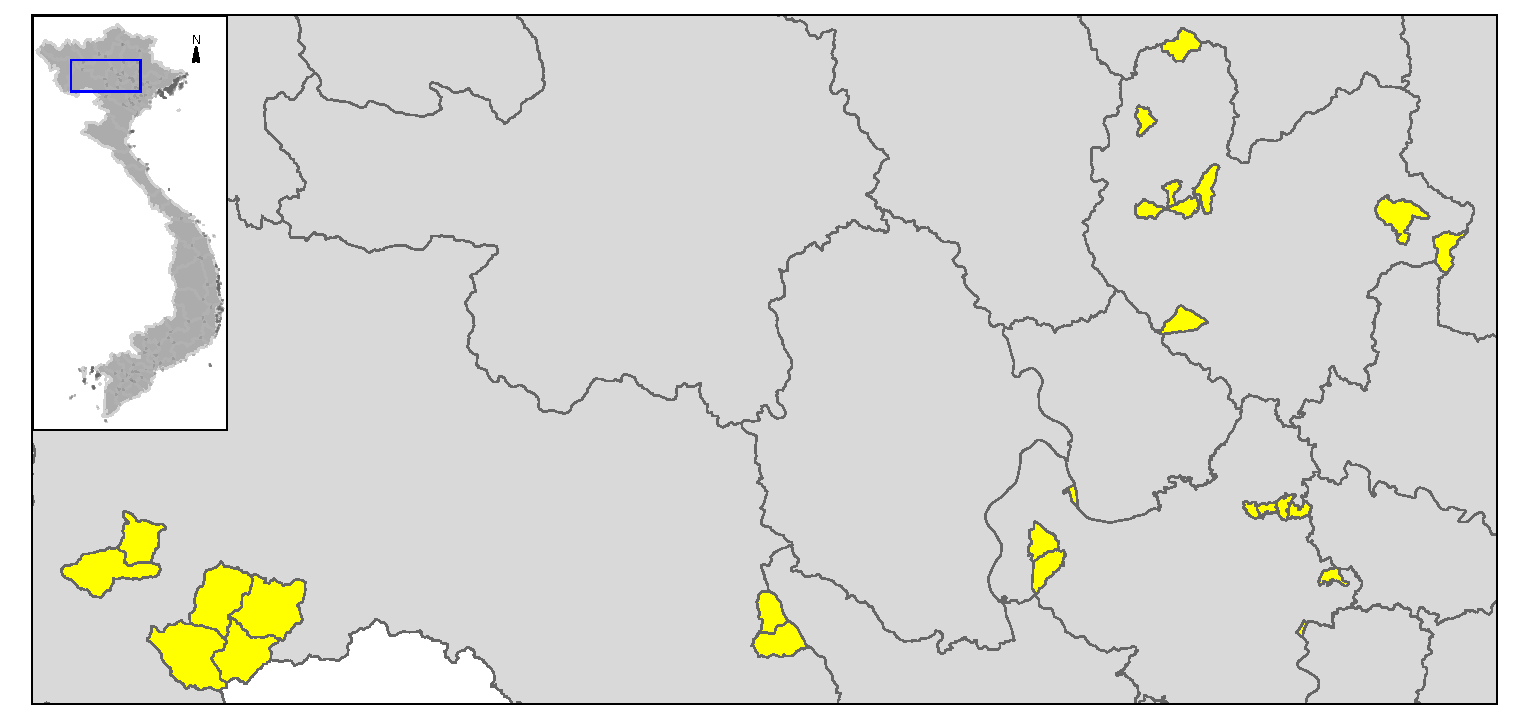
\includegraphics[width=1\textwidth]{map01.pdf}
\end{center}
\end{frame}

\begin{frame}
% latex table generated in R 4.2.1 by xtable 1.8-4 package
% Thu Oct 12 12:55:24 2023
\begin{table}[ht]
\centering
{\tiny%
\begin{tabular}{lrrrr}
  \toprule
Commune & summer & autumn & winter & spring \\
  \midrule
Bac Hong &   0 &   0 &   0 & 100 \\
  Binh Long &   0 &   0 & 100 &   0 \\
  Cat Ne &   0 & 100 &   0 &   0 \\
  Chieng Cang &   0 & 100 &   0 &   0 \\
  Chieng Khoong & 100 &   0 &   0 &   0 \\
  Chieng So &   0 &   0 &   0 &  85 \\
  Dong Dat &   0 &   0 &   0 &  99 \\
  Dong Thinh & 100 &   0 &   0 &   0 \\
  Duc Luong &   0 & 100 &   0 &   0 \\
  Hop Thanh &   0 &   0 &   0 & 101 \\
  Kim Lan &   0 & 100 &   0 &   0 \\
  Lien Hoa &   0 &   0 & 100 &   0 \\
  Linh Thong & 100 &   0 &   0 &   0 \\
  Minh Chau &  56 &   0 &   0 &   0 \\
  Muong Cai &   0 & 100 &   0 &   0 \\
  Muong Hung & 100 &   0 &   0 &   0 \\
  Nam Man &   0 &   0 &   0 & 115 \\
  Nguyen Khe &   0 &   0 &   0 & 100 \\
  Phu Dong &  82 &   0 &   0 &   0 \\
  Song Khua &   0 &   0 & 100 &   0 \\
  Tan Linh &  62 &  50 &   0 &   0 \\
  Thuy Lam &   0 &   0 & 100 &   0 \\
  Trang &   0 &   0 & 100 &   0 \\
  Van Hoa &   0 &  50 &   0 &   0 \\
  Xuan Non &   0 &   0 & 100 &   0 \\
   \bottomrule
\end{tabular}}
\end{table}
\end{frame}


\begin{frame}
\begin{center}
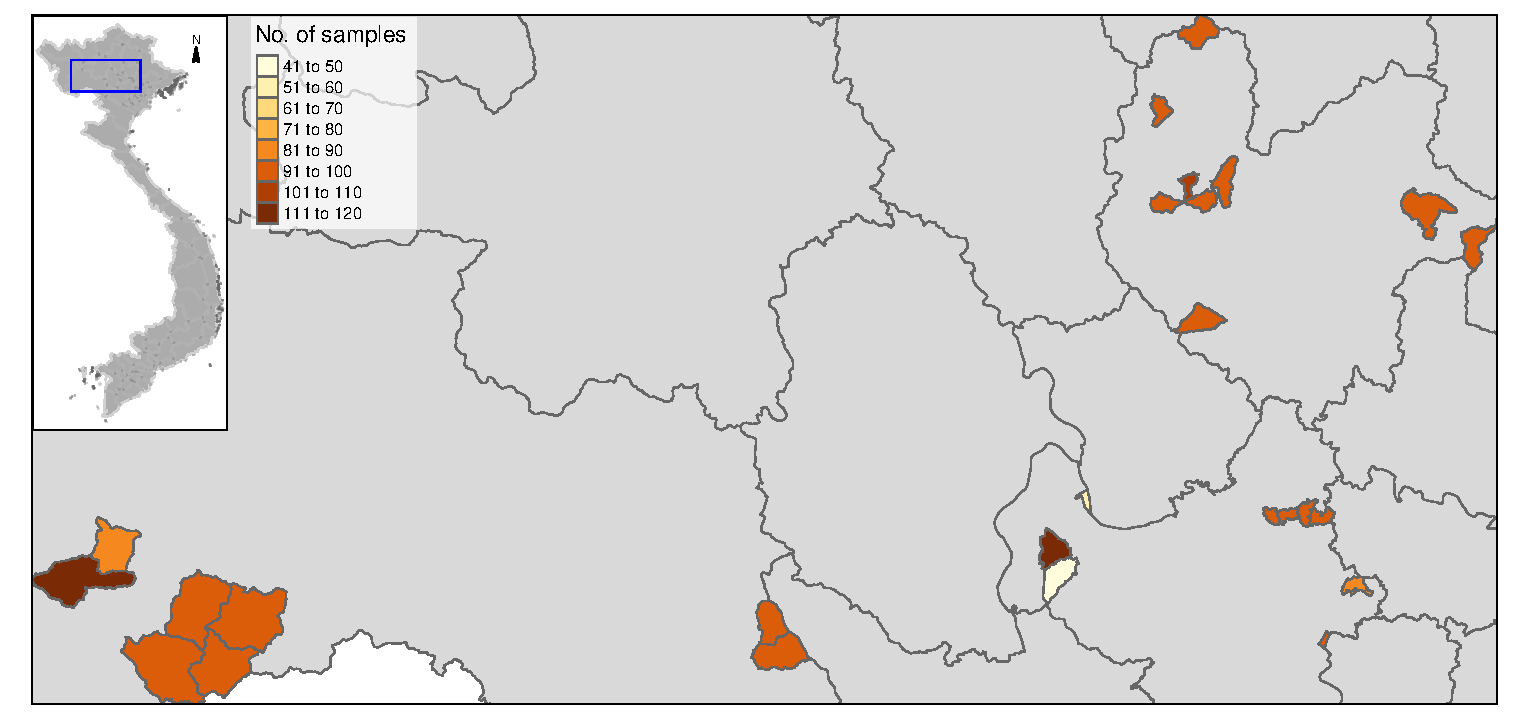
\includegraphics[width=1\textwidth]{map02.pdf}
\end{center}
\end{frame}

\begin{frame}
summer\\
\begin{center}
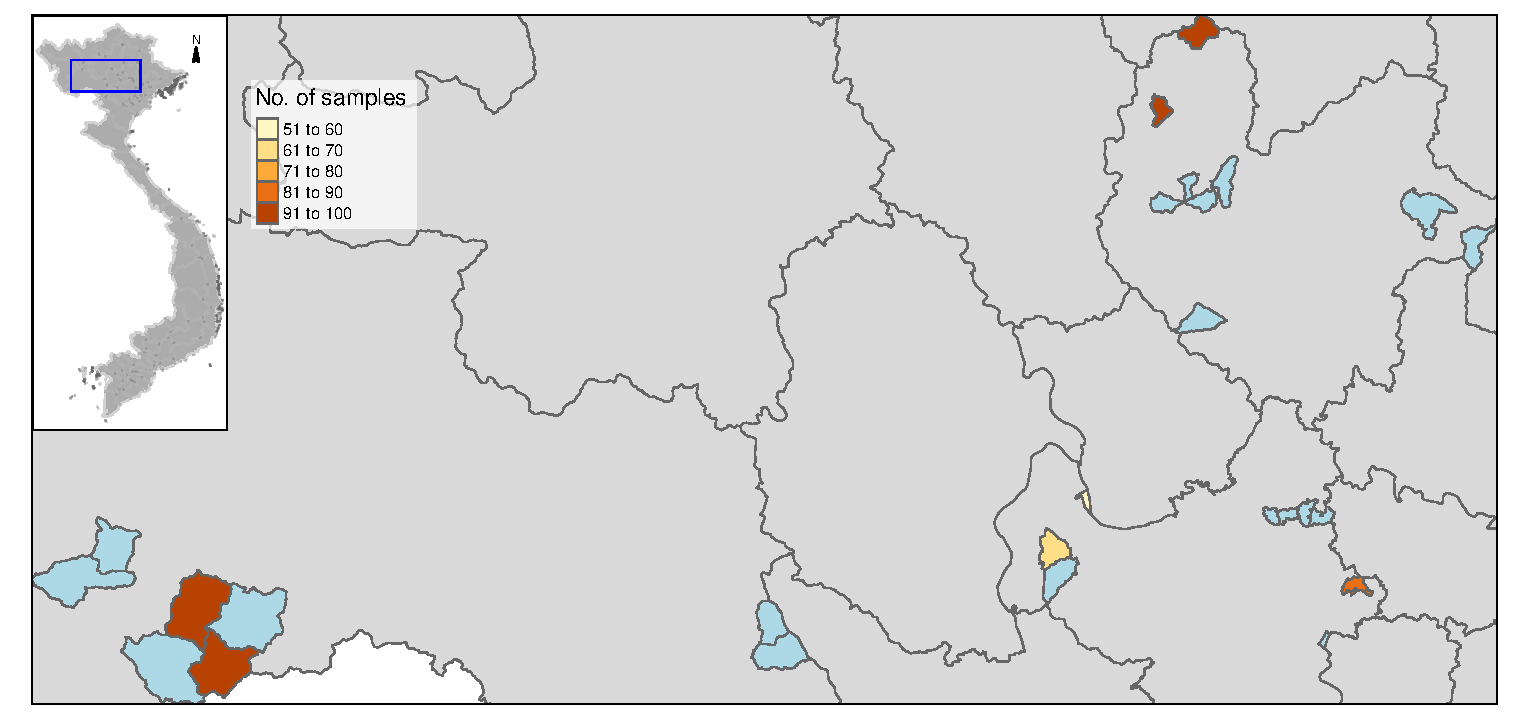
\includegraphics[width=1\textwidth]{map02_summer.pdf}
\end{center}
\end{frame}


\begin{frame}
autumn\\
\begin{center}
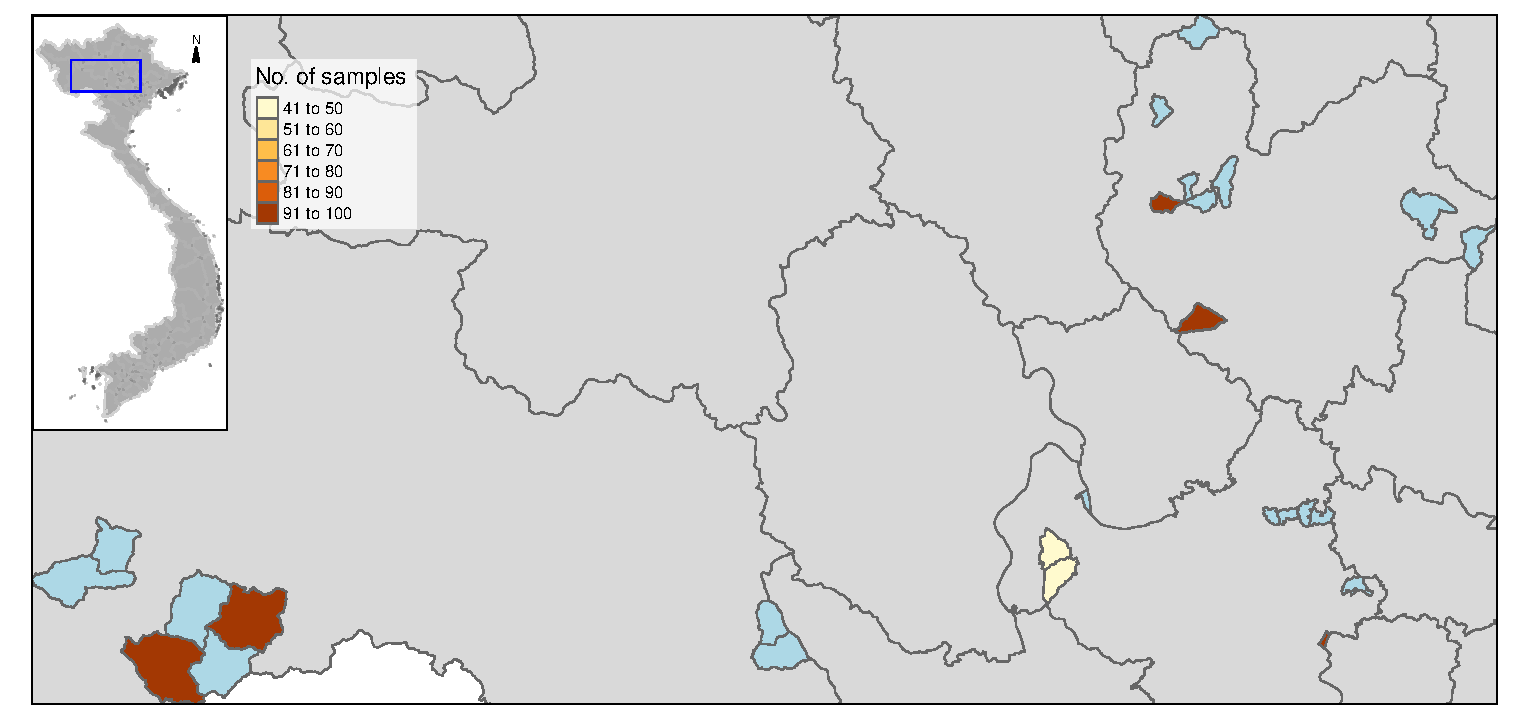
\includegraphics[width=1\textwidth]{map02_autumn.pdf}
\end{center}
\end{frame}

\begin{frame}
winter\\
\begin{center}
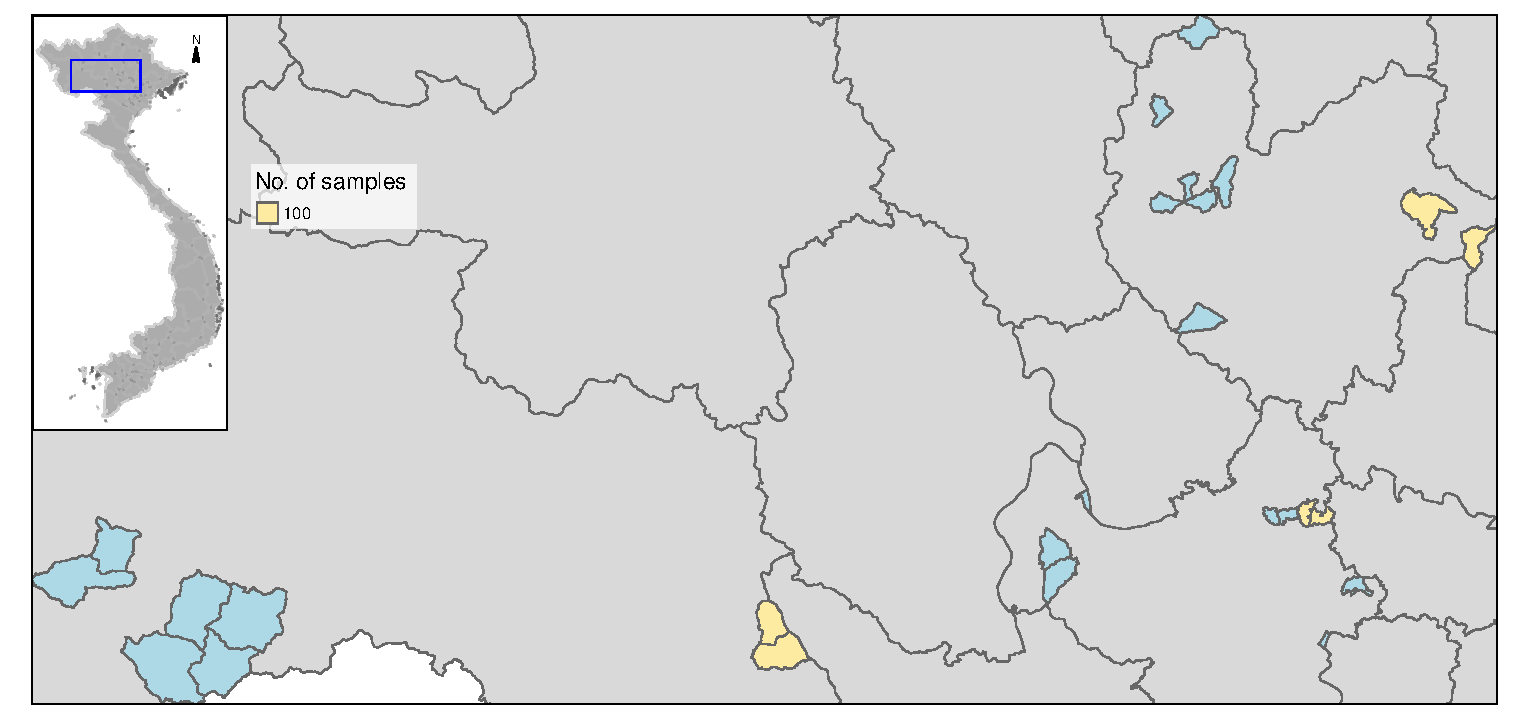
\includegraphics[width=1\textwidth]{map02_winter.pdf}
\end{center}
\end{frame}


\begin{frame}
spring\\
\begin{center}
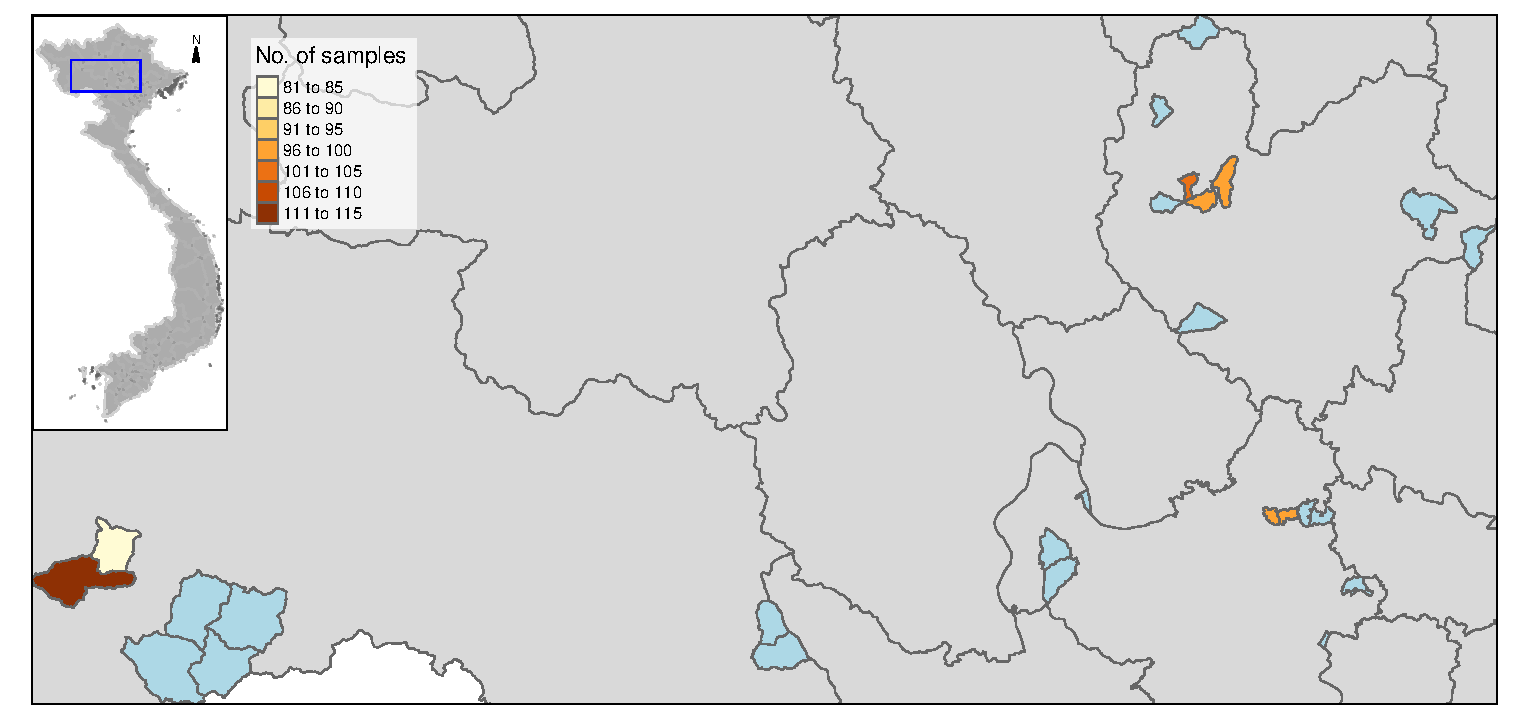
\includegraphics[width=1\textwidth]{map02_spring.pdf}
\end{center}
\end{frame}

\section{Prevalence}
\begin{frame}
\begin{center}
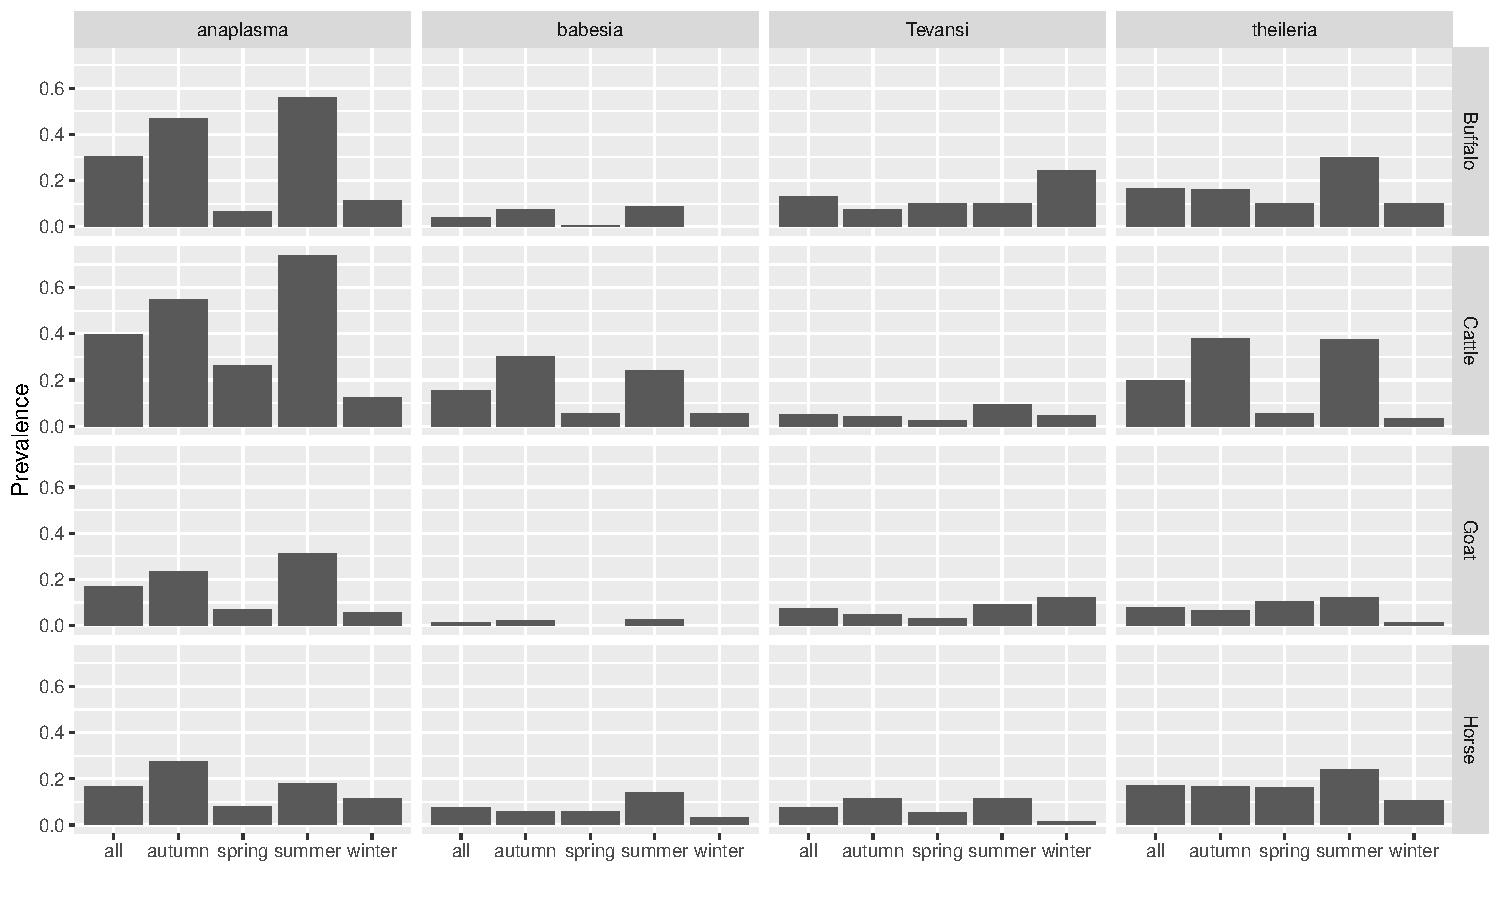
\includegraphics[width=1\textwidth]{fig_prev01.pdf}
\end{center}
\end{frame}


\subsection{Anaplasma}
\begin{frame}
\begin{center}
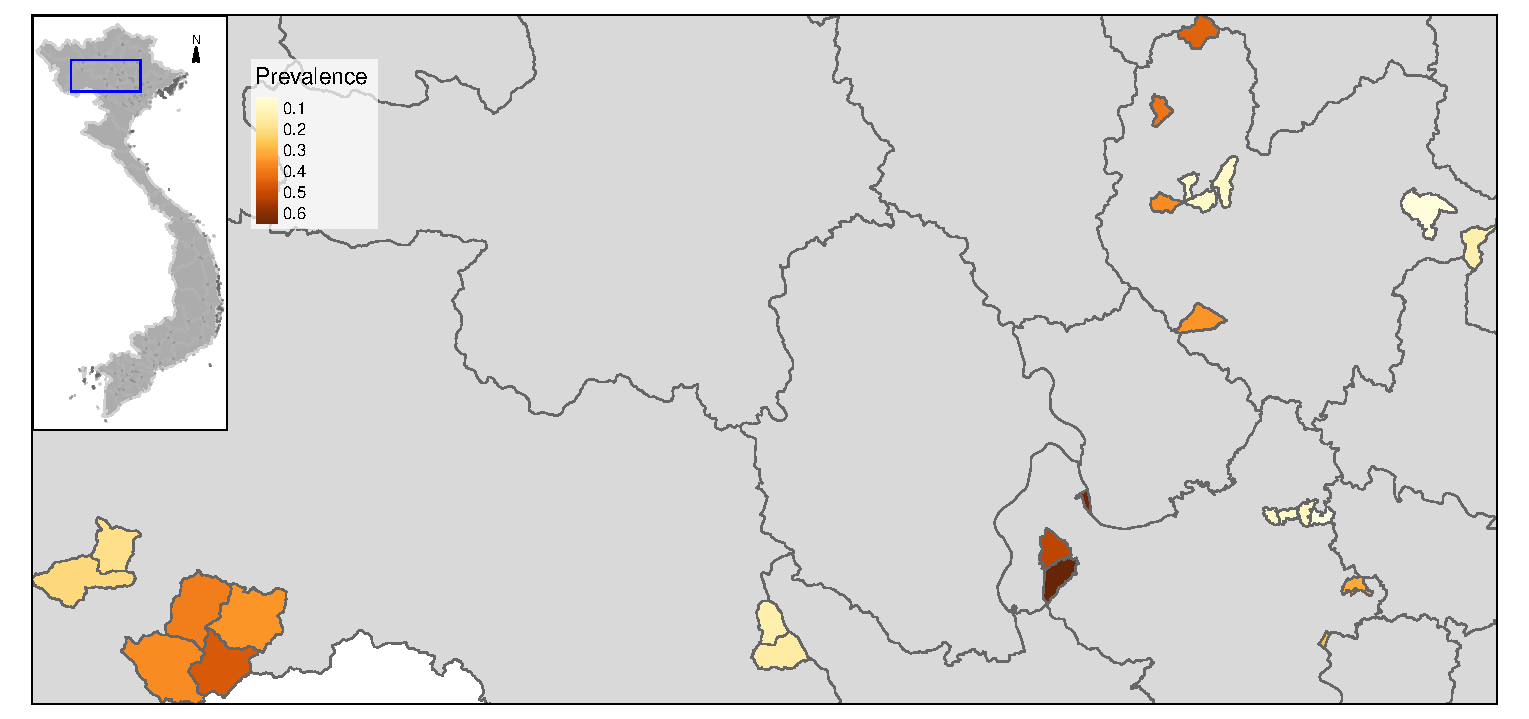
\includegraphics[width=1\textwidth]{map03.pdf}
\end{center}
\end{frame}

\begin{frame}
summer\\
\begin{center}
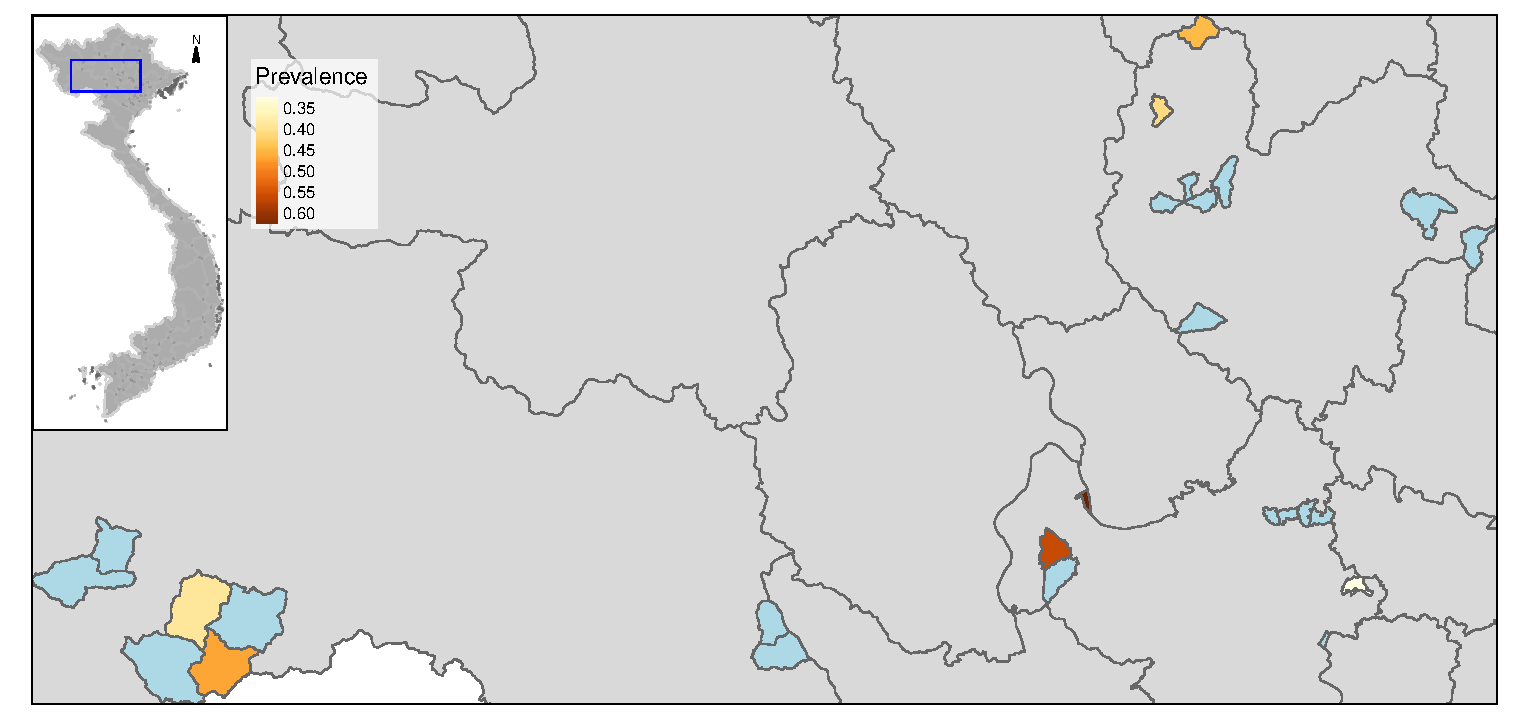
\includegraphics[width=1\textwidth]{map03_summer.pdf}
\end{center}
\end{frame}


\begin{frame}
autumn\\
\begin{center}
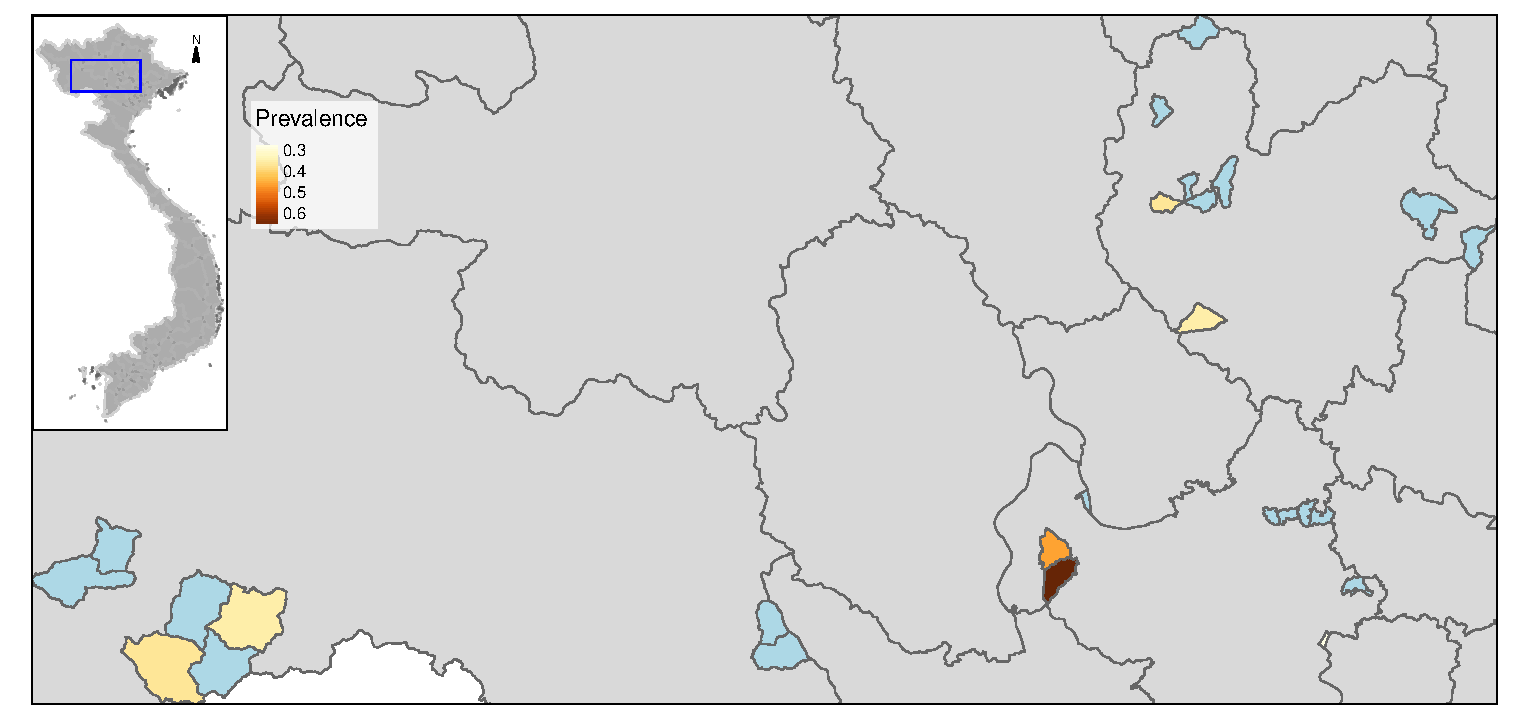
\includegraphics[width=1\textwidth]{map03_autumn.pdf}
\end{center}
\end{frame}

\begin{frame}
winter\\
\begin{center}
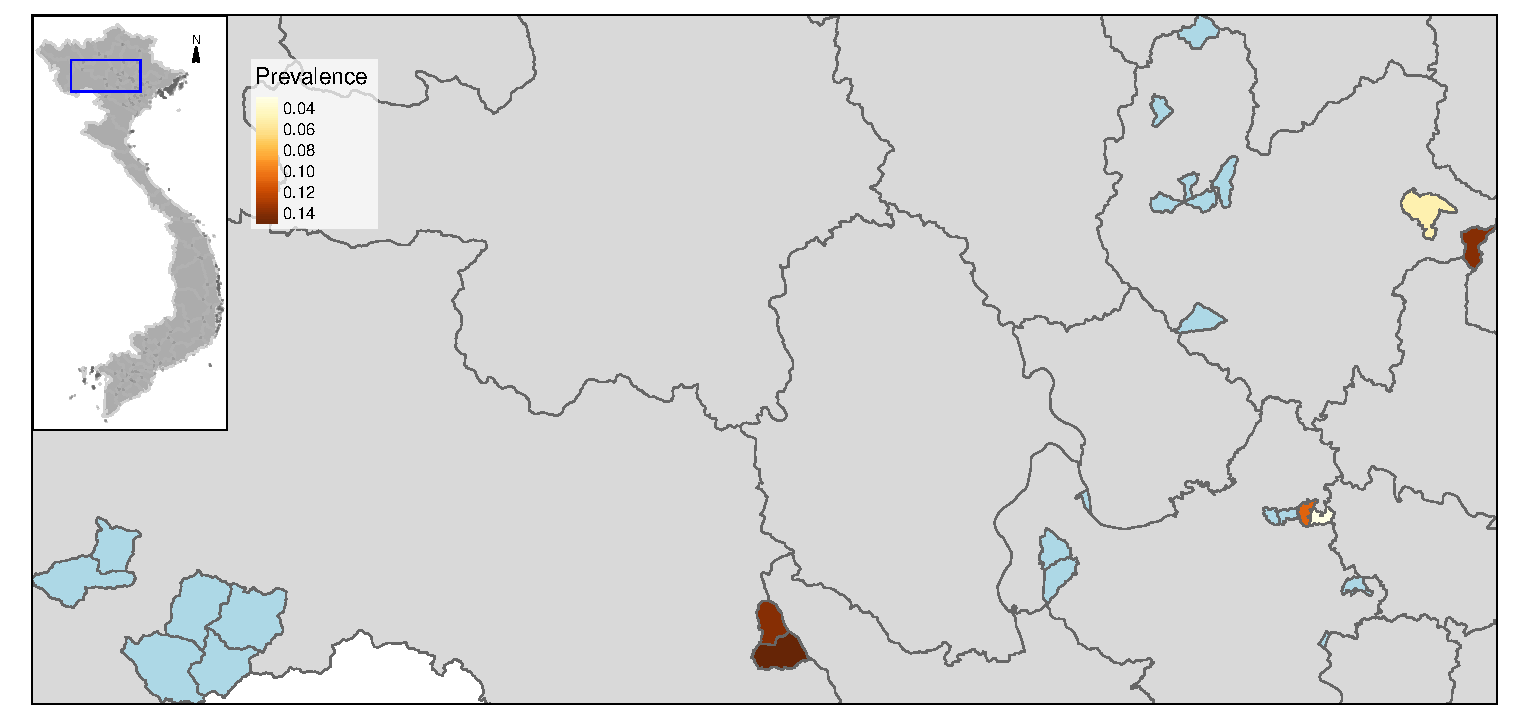
\includegraphics[width=1\textwidth]{map03_winter.pdf}
\end{center}
\end{frame}


\begin{frame}
spring\\
\begin{center}
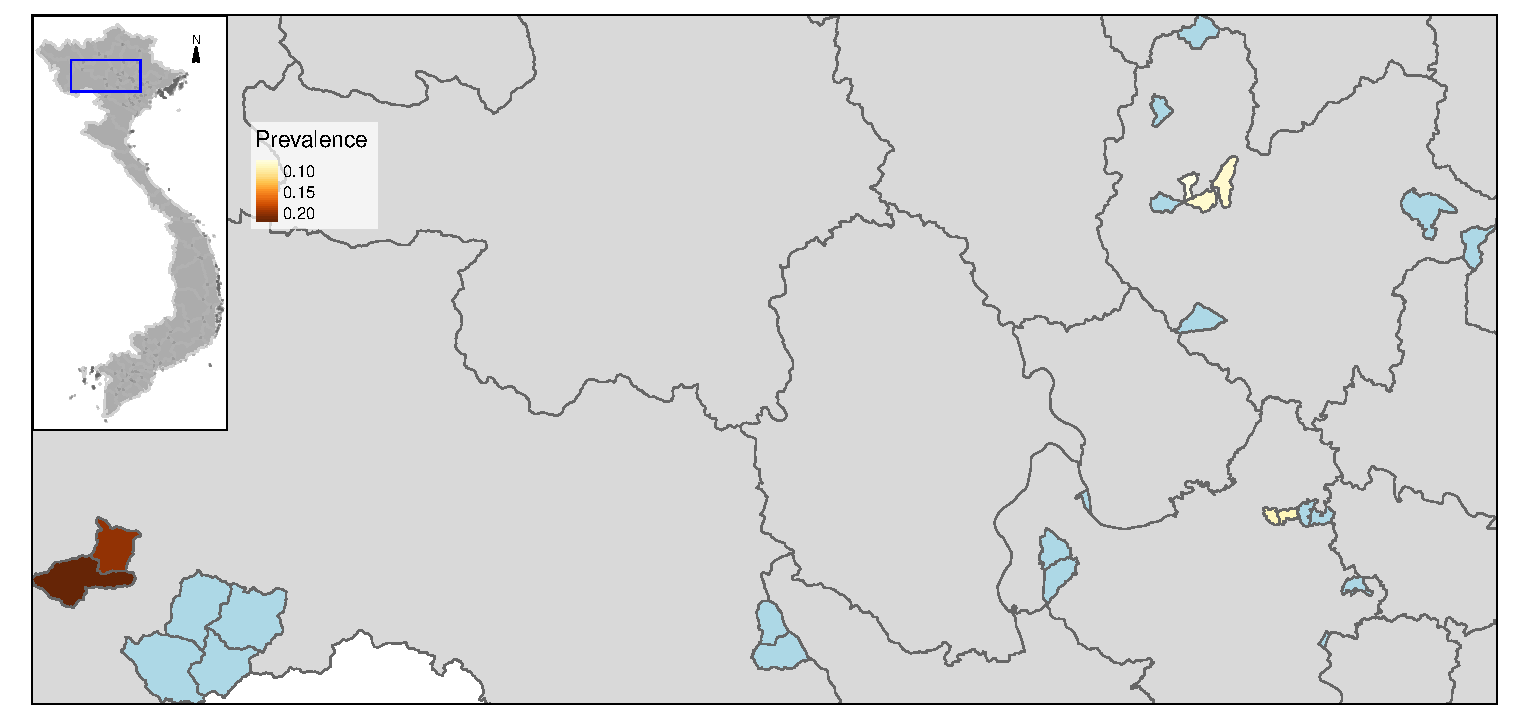
\includegraphics[width=1\textwidth]{map03_spring.pdf}
\end{center}
\end{frame}

\subsection{Babesia}
\begin{frame}
\begin{center}
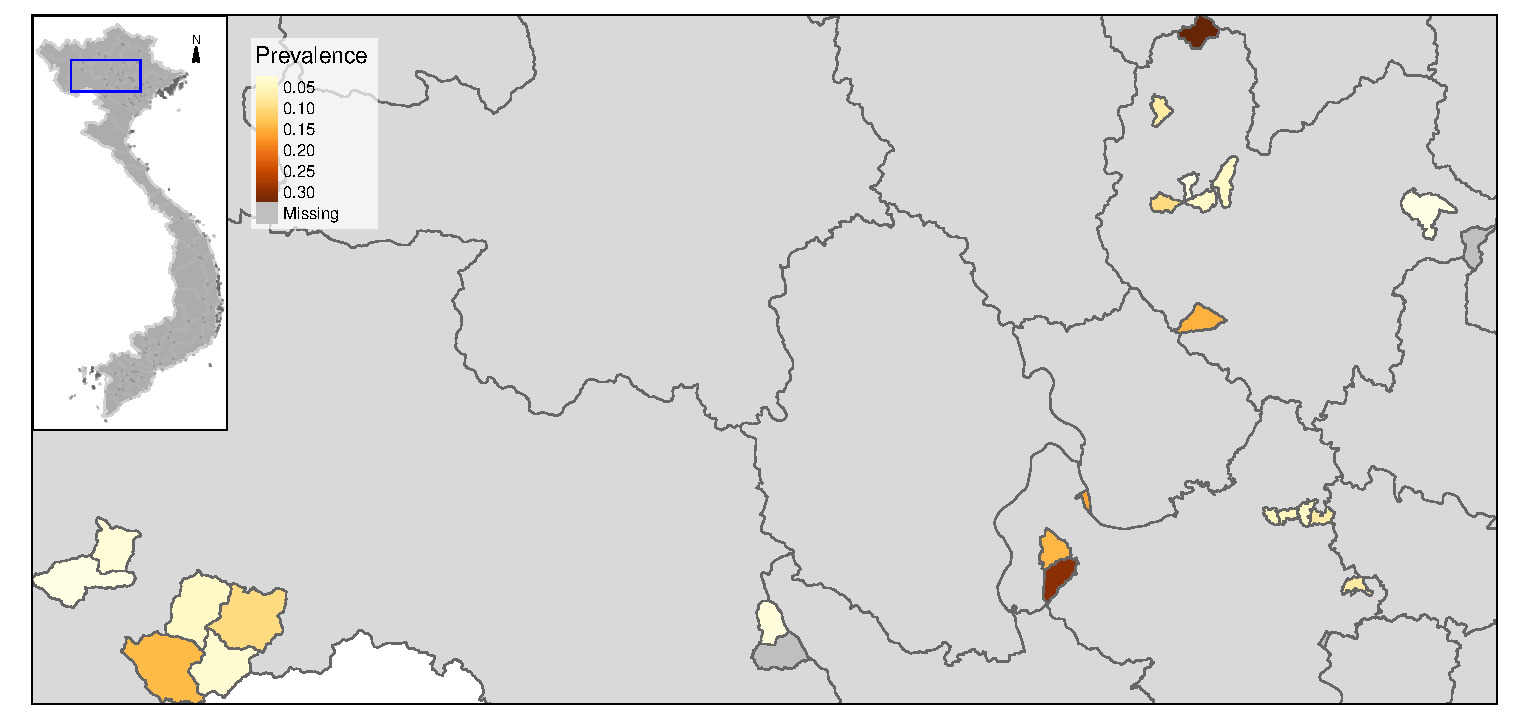
\includegraphics[width=1\textwidth]{map04.pdf}
\end{center}
\end{frame}

\begin{frame}
summer\\
\begin{center}
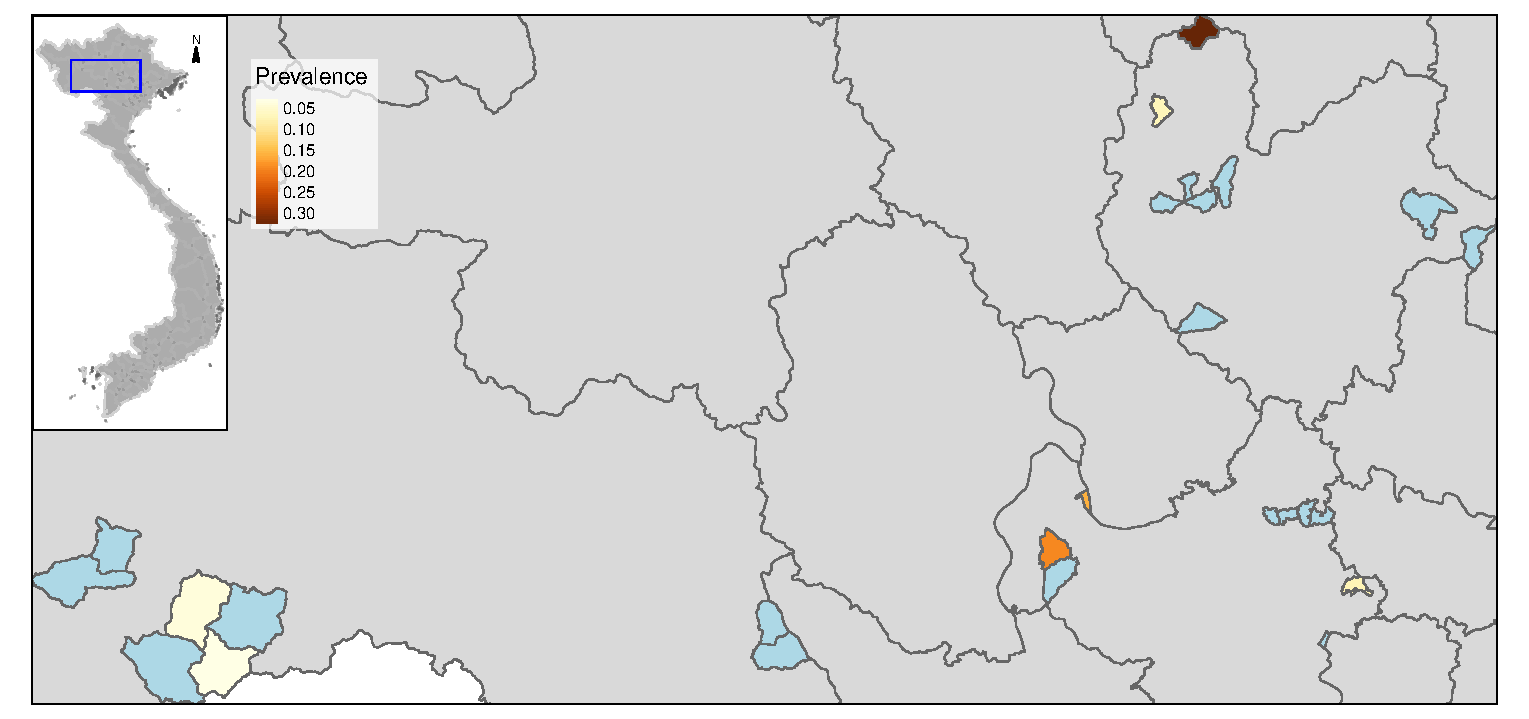
\includegraphics[width=1\textwidth]{map04_summer.pdf}
\end{center}
\end{frame}


\begin{frame}
autumn\\
\begin{center}
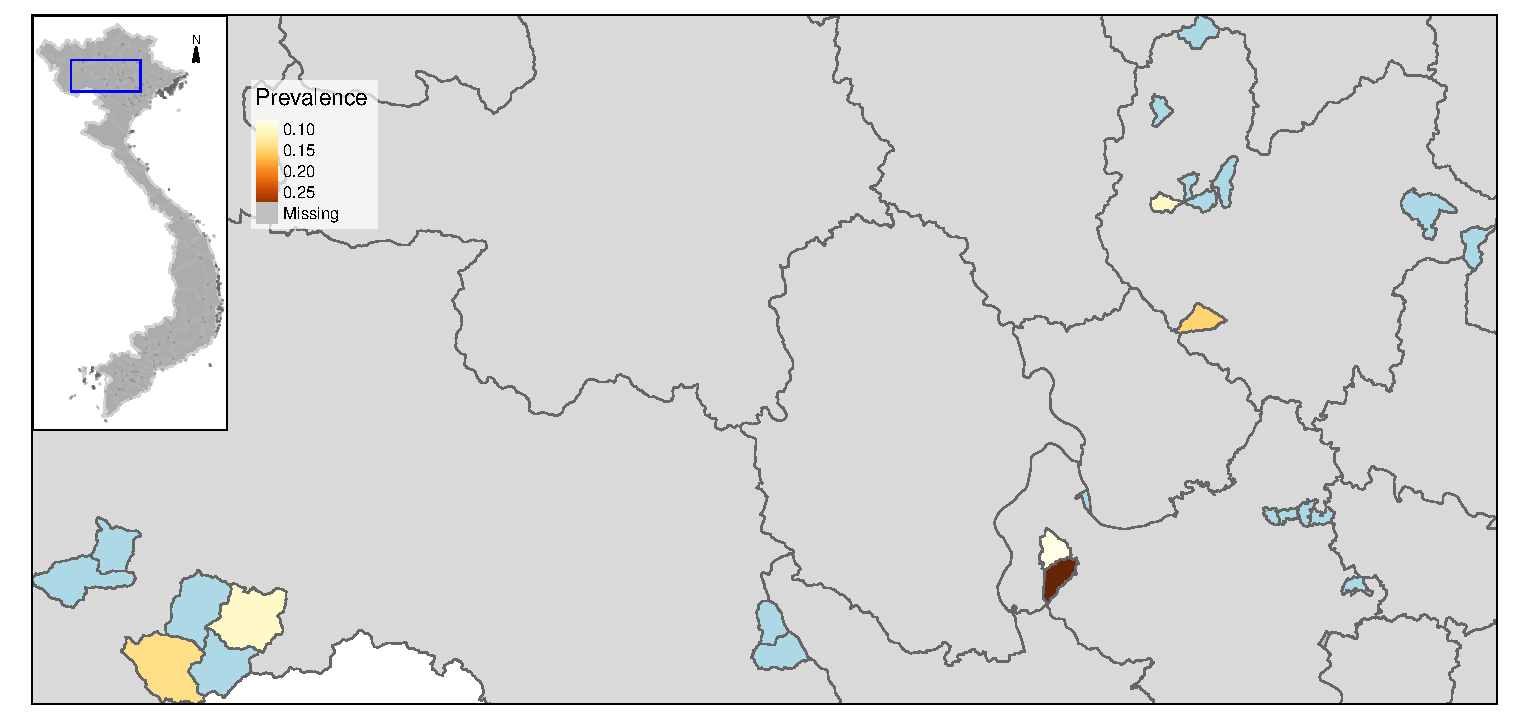
\includegraphics[width=1\textwidth]{map04_autumn.pdf}
\end{center}
\end{frame}

\begin{frame}
winter\\
\begin{center}
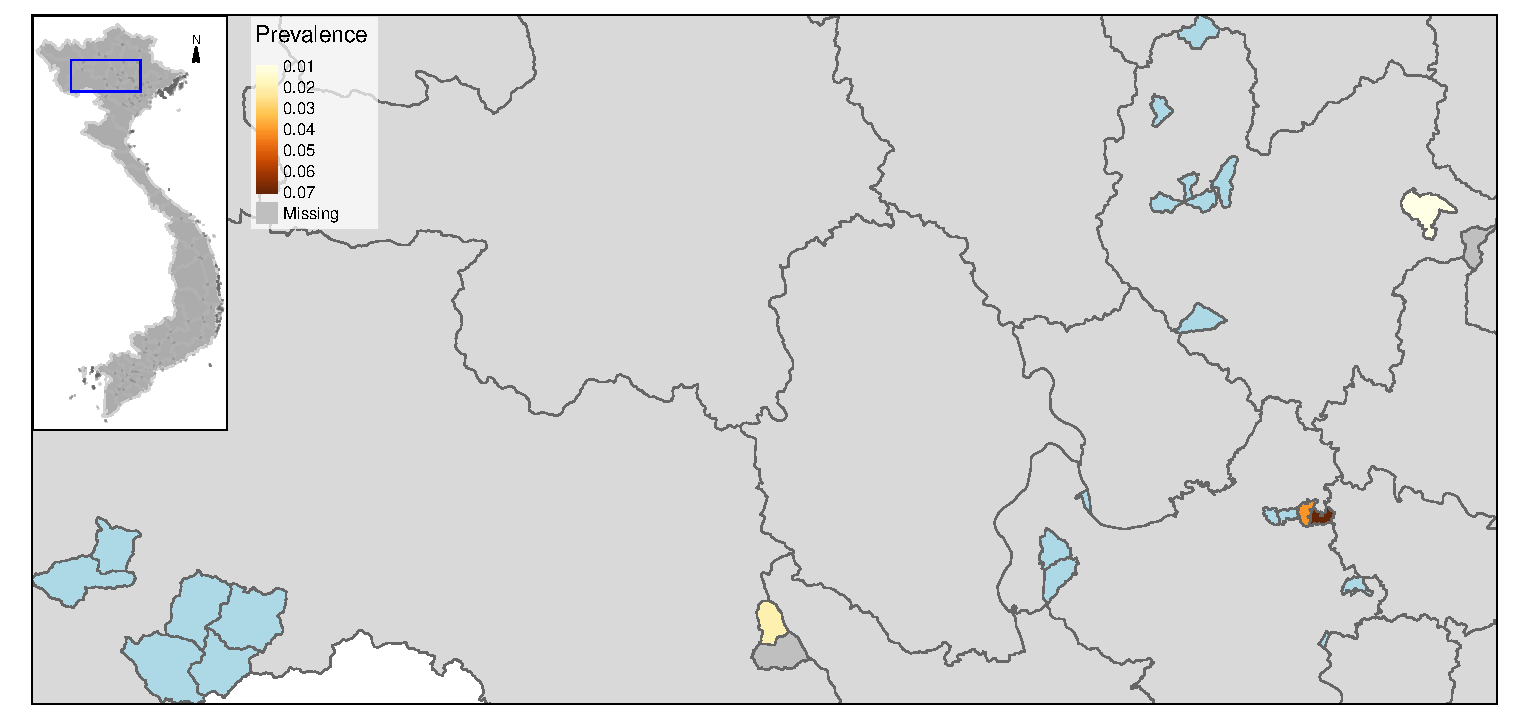
\includegraphics[width=1\textwidth]{map04_winter.pdf}
\end{center}
\end{frame}


\begin{frame}
spring\\
\begin{center}
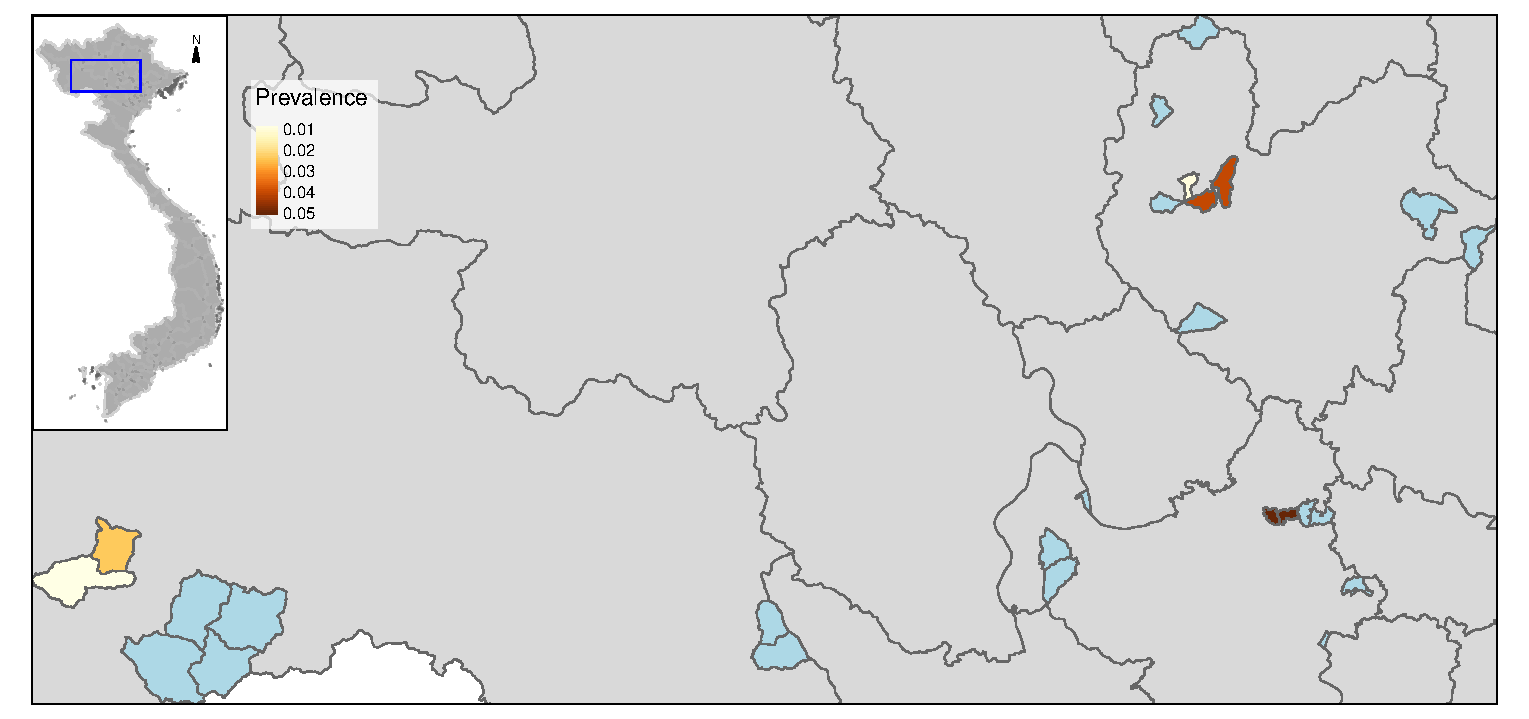
\includegraphics[width=1\textwidth]{map04_spring.pdf}
\end{center}
\end{frame}


\subsection{Theileria}
\begin{frame}
\begin{center}
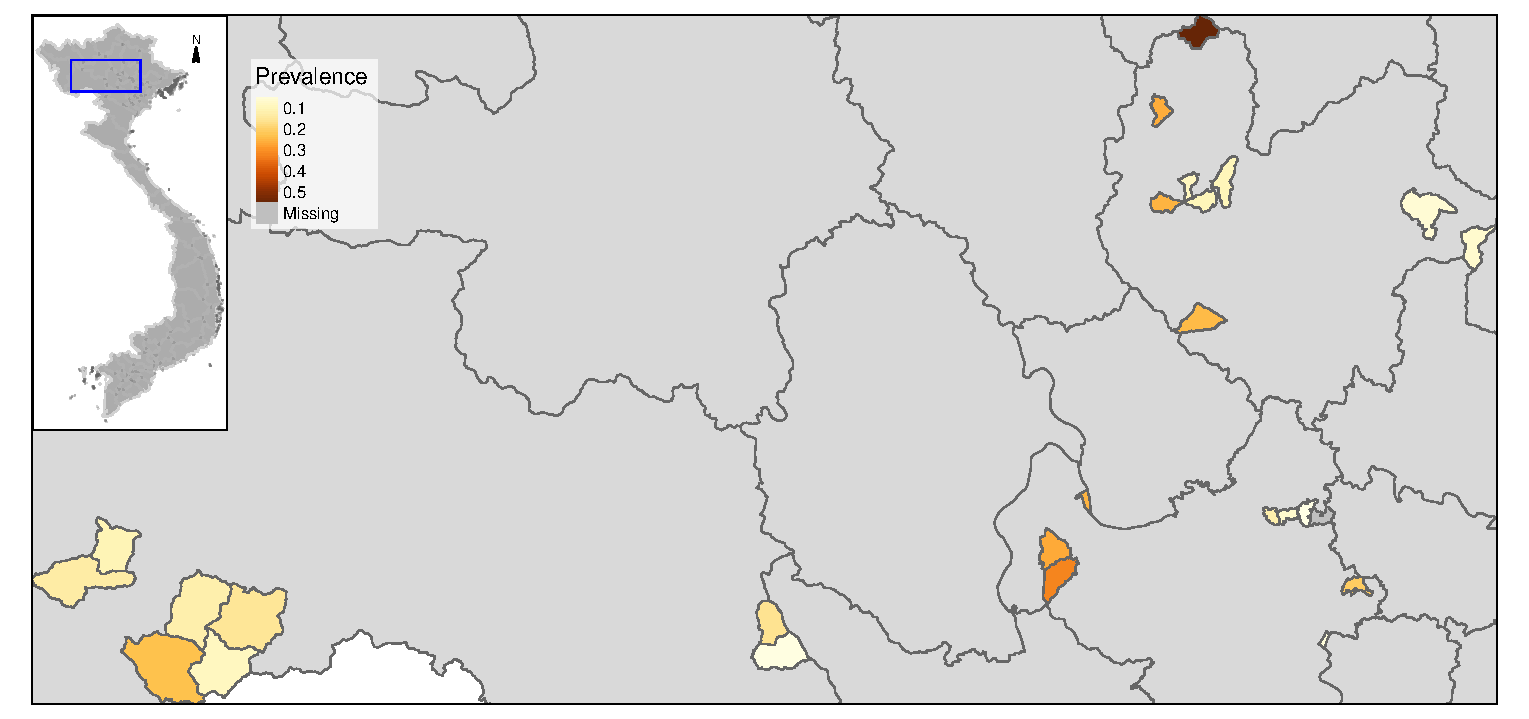
\includegraphics[width=1\textwidth]{map05.pdf}
\end{center}
\end{frame}

\begin{frame}
summer\\
\begin{center}
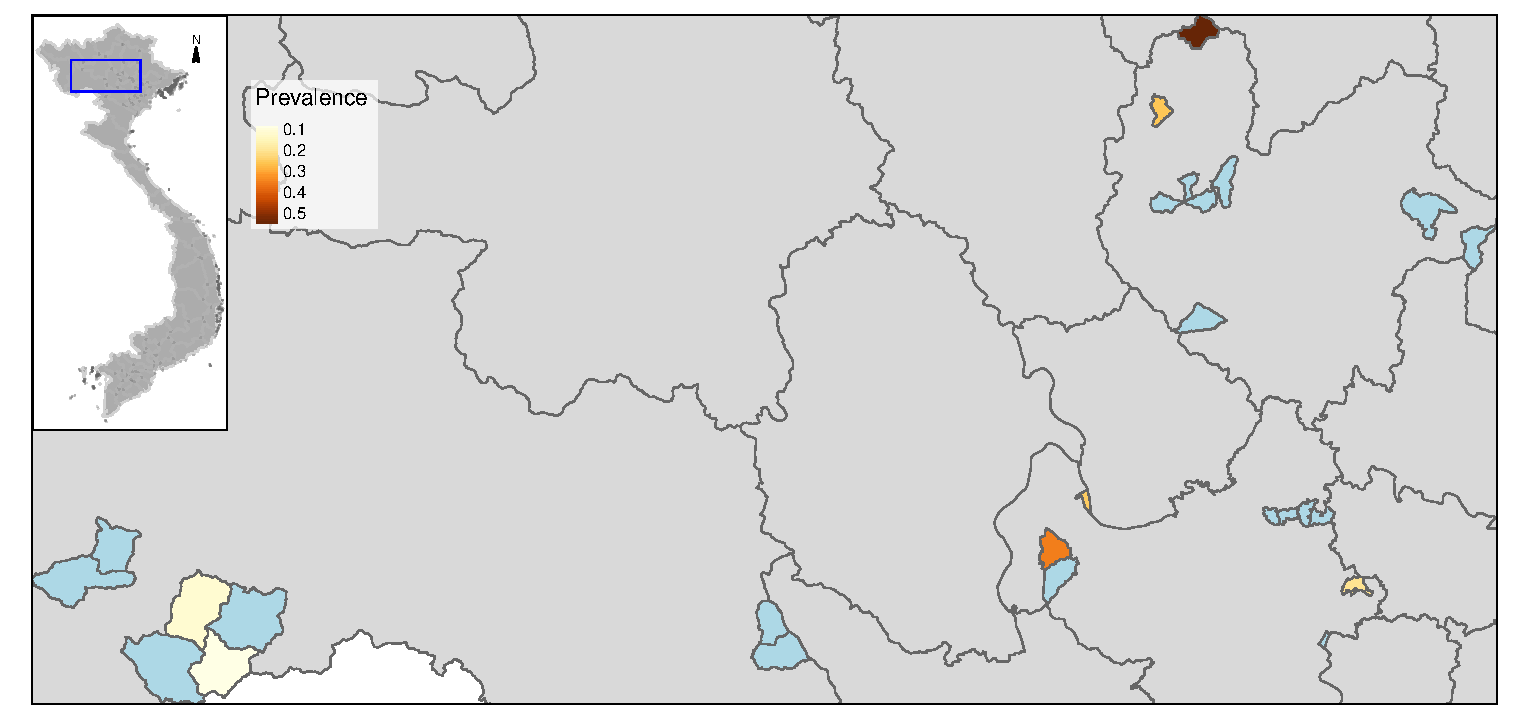
\includegraphics[width=1\textwidth]{map05_summer.pdf}
\end{center}
\end{frame}


\begin{frame}
autumn\\
\begin{center}
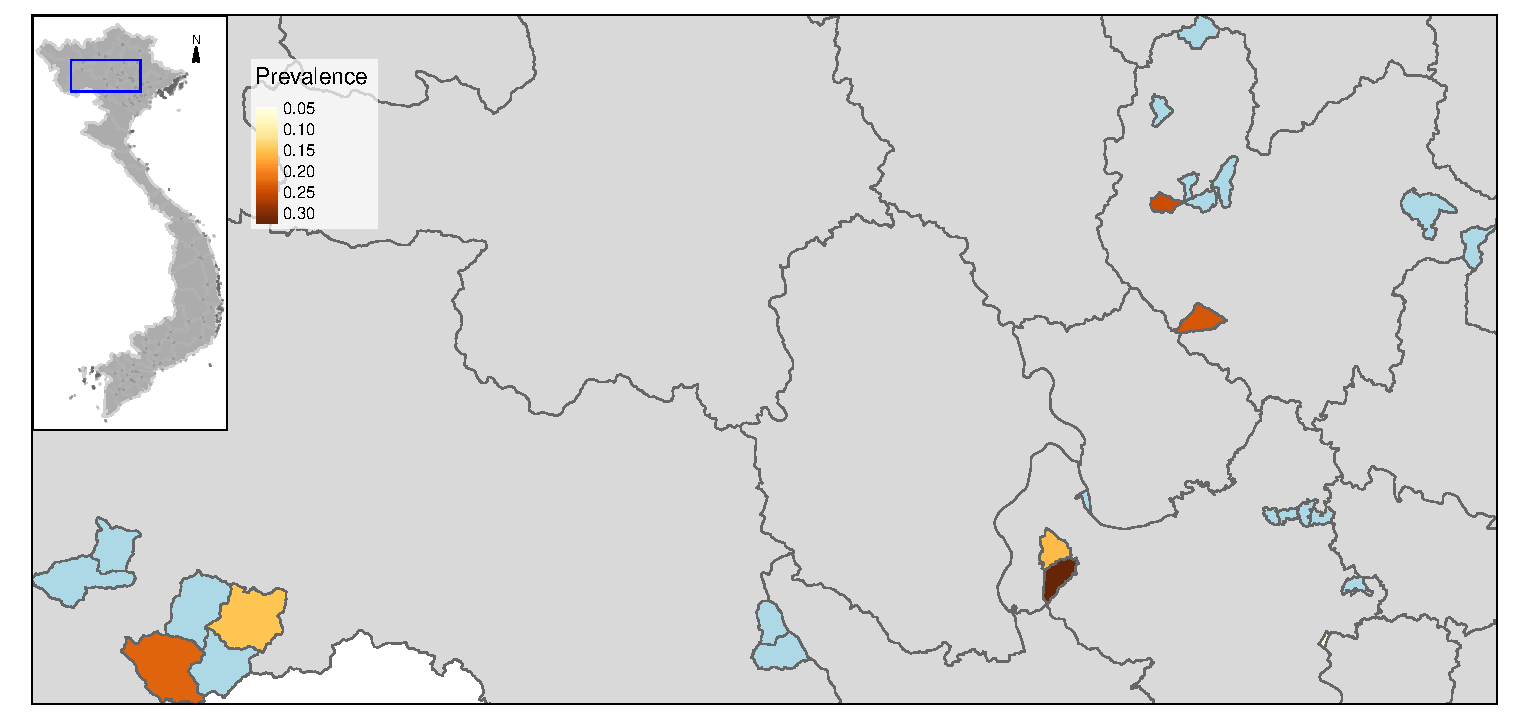
\includegraphics[width=1\textwidth]{map05_autumn.pdf}
\end{center}
\end{frame}

\begin{frame}
winter\\
\begin{center}
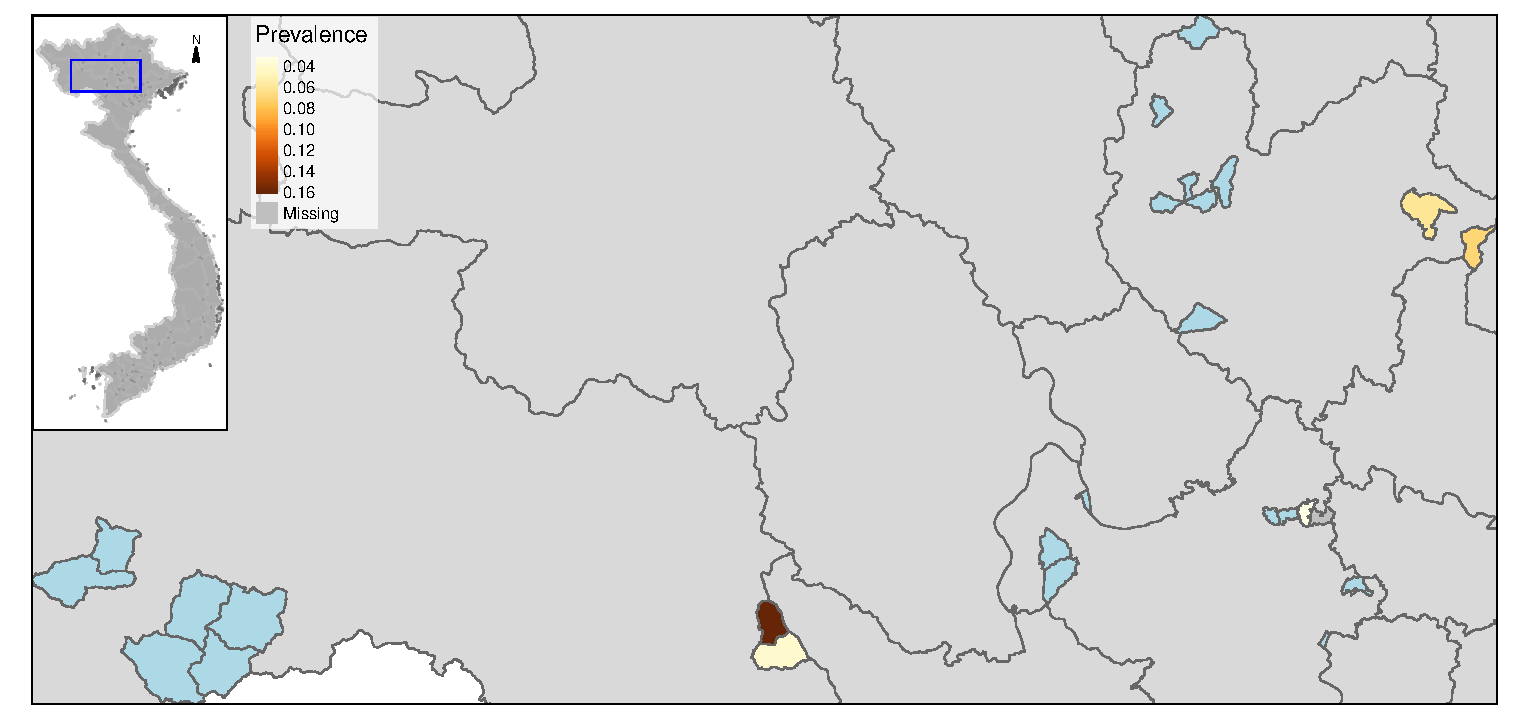
\includegraphics[width=1\textwidth]{map05_winter.pdf}
\end{center}
\end{frame}


\begin{frame}
spring\\
\begin{center}
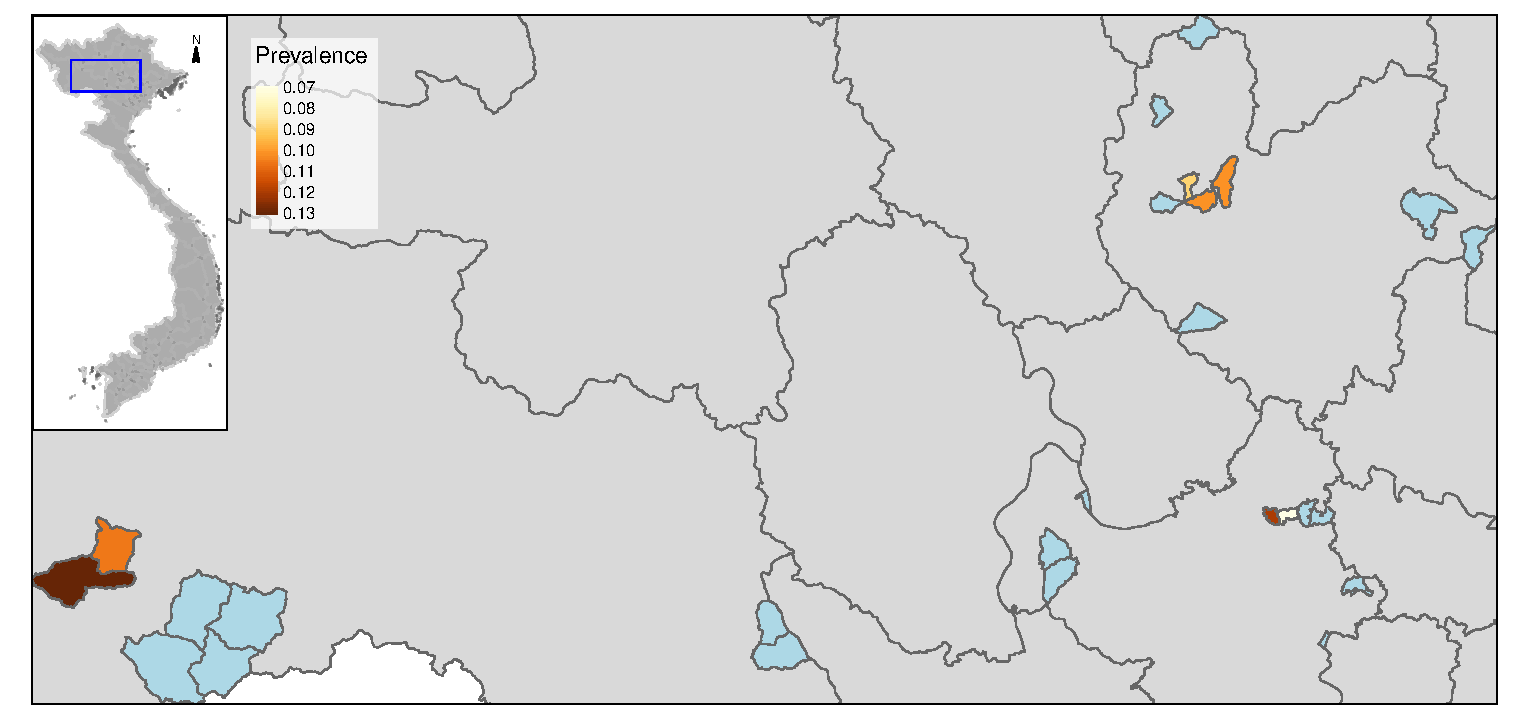
\includegraphics[width=1\textwidth]{map05_spring.pdf}
\end{center}
\end{frame}


\subsection{\textit{Trypanosoma evansi}}
\begin{frame}
\begin{center}
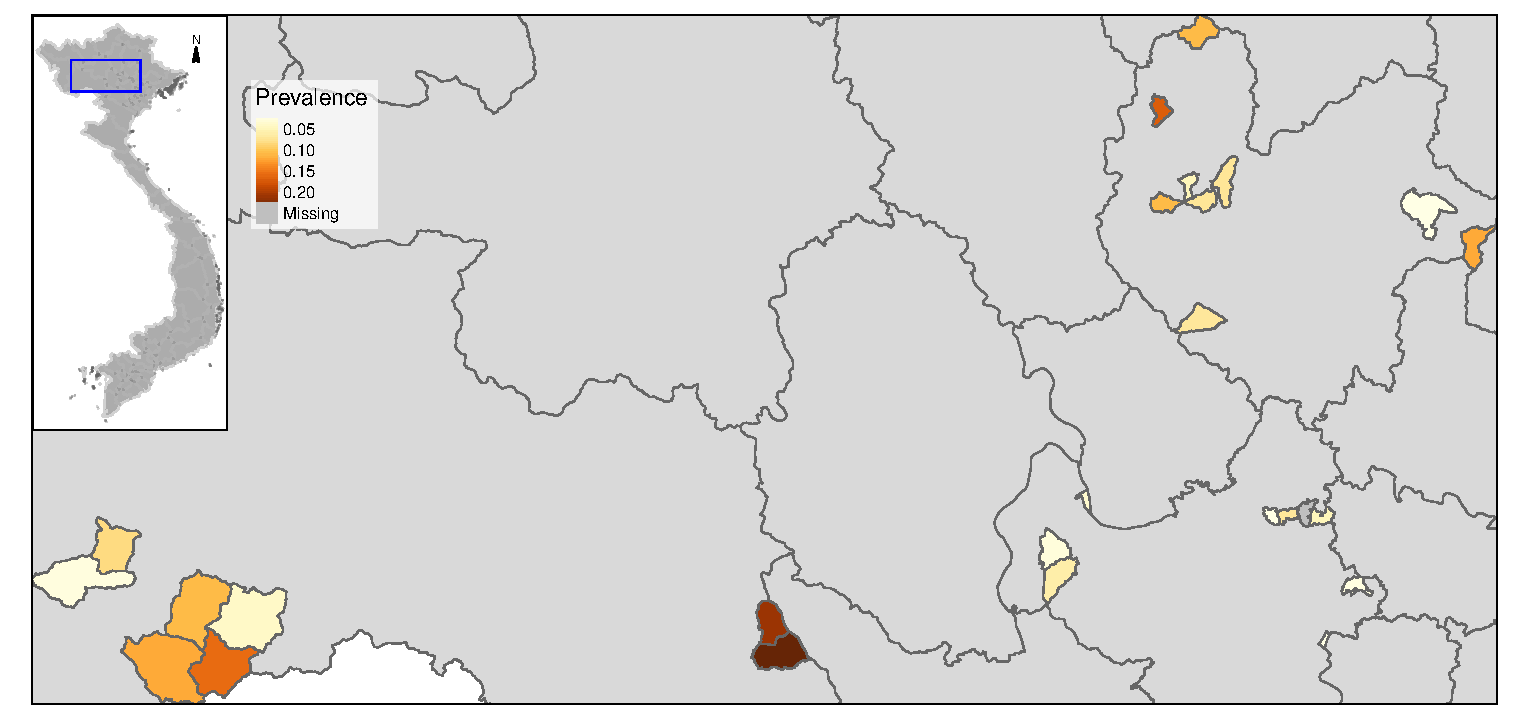
\includegraphics[width=1\textwidth]{map06.pdf}
\end{center}
\end{frame}

\begin{frame}
summer\\
\begin{center}
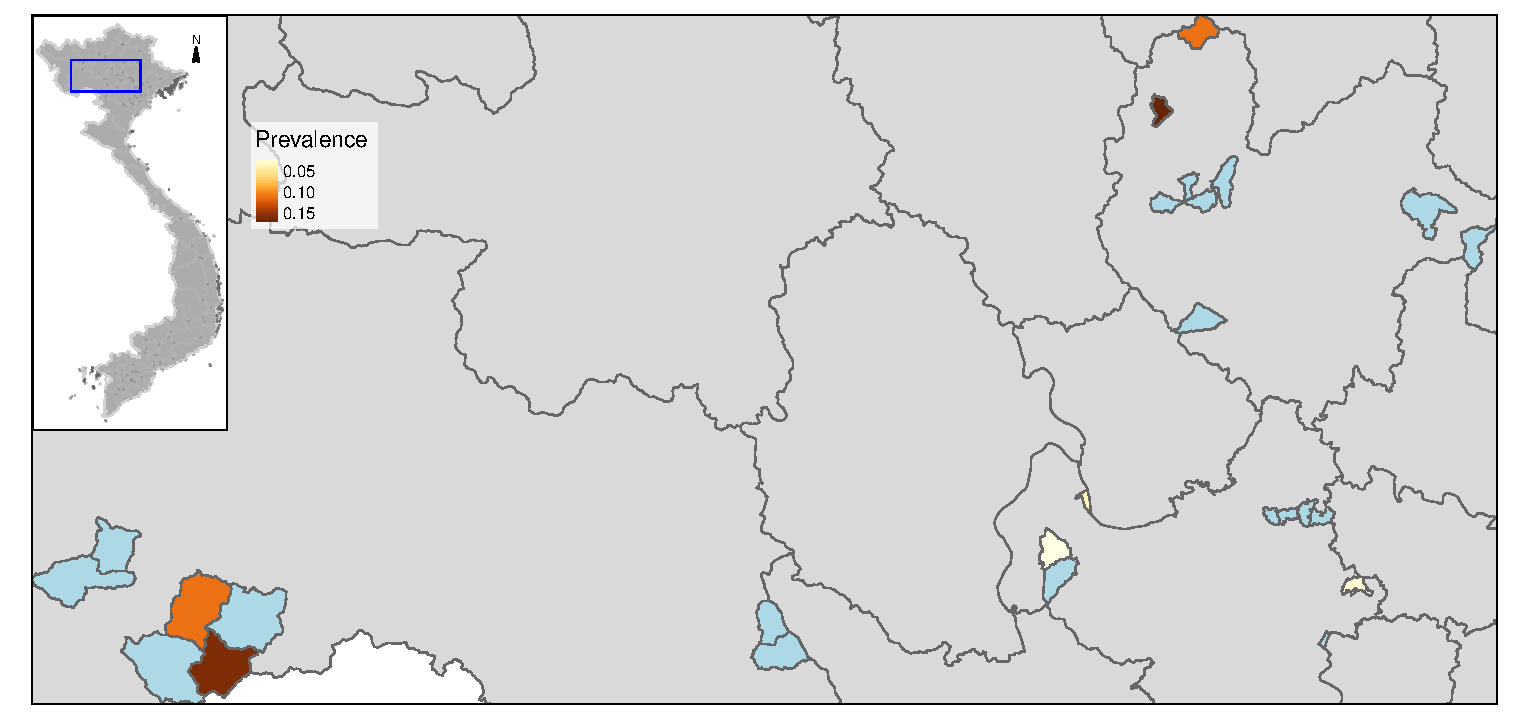
\includegraphics[width=1\textwidth]{map06_summer.pdf}
\end{center}
\end{frame}


\begin{frame}
autumn\\
\begin{center}
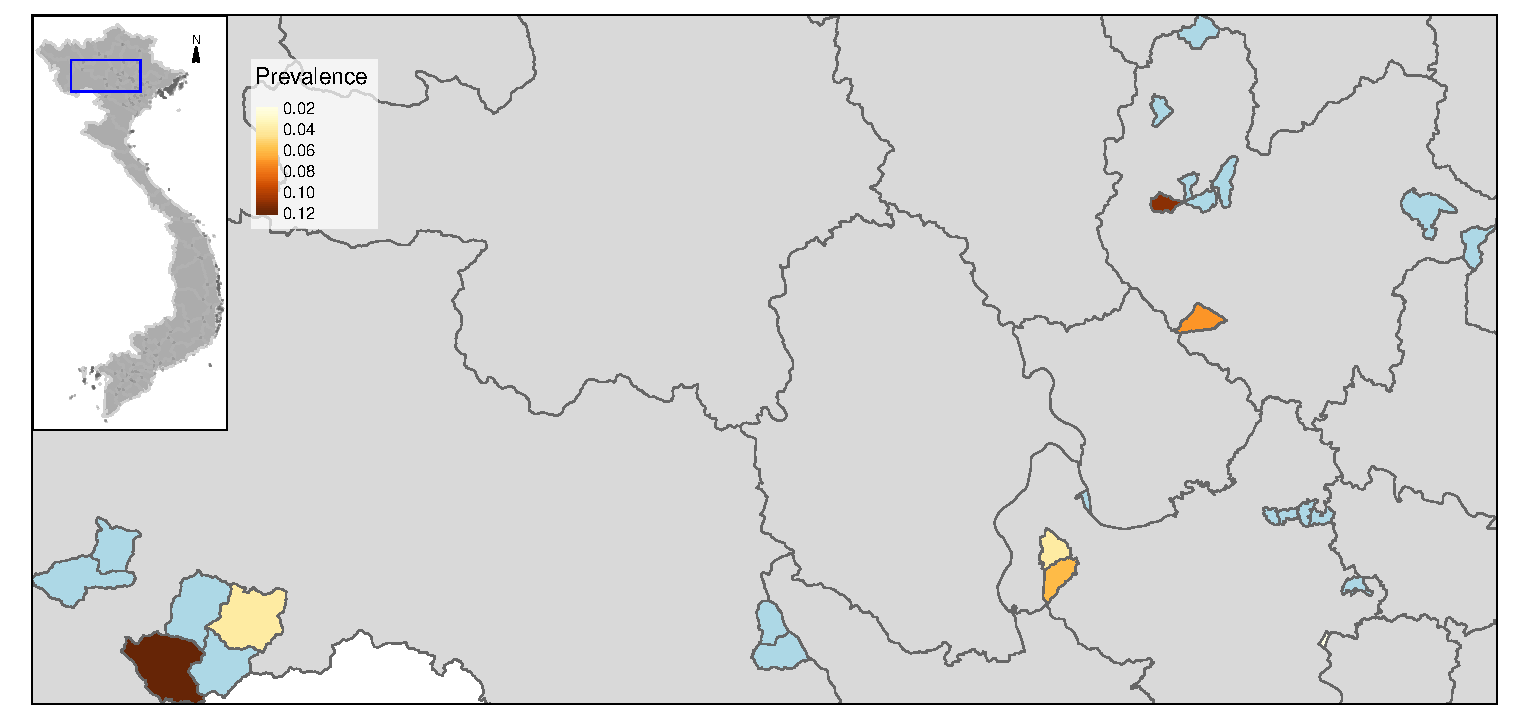
\includegraphics[width=1\textwidth]{map06_autumn.pdf}
\end{center}
\end{frame}

\begin{frame}
winter\\
\begin{center}
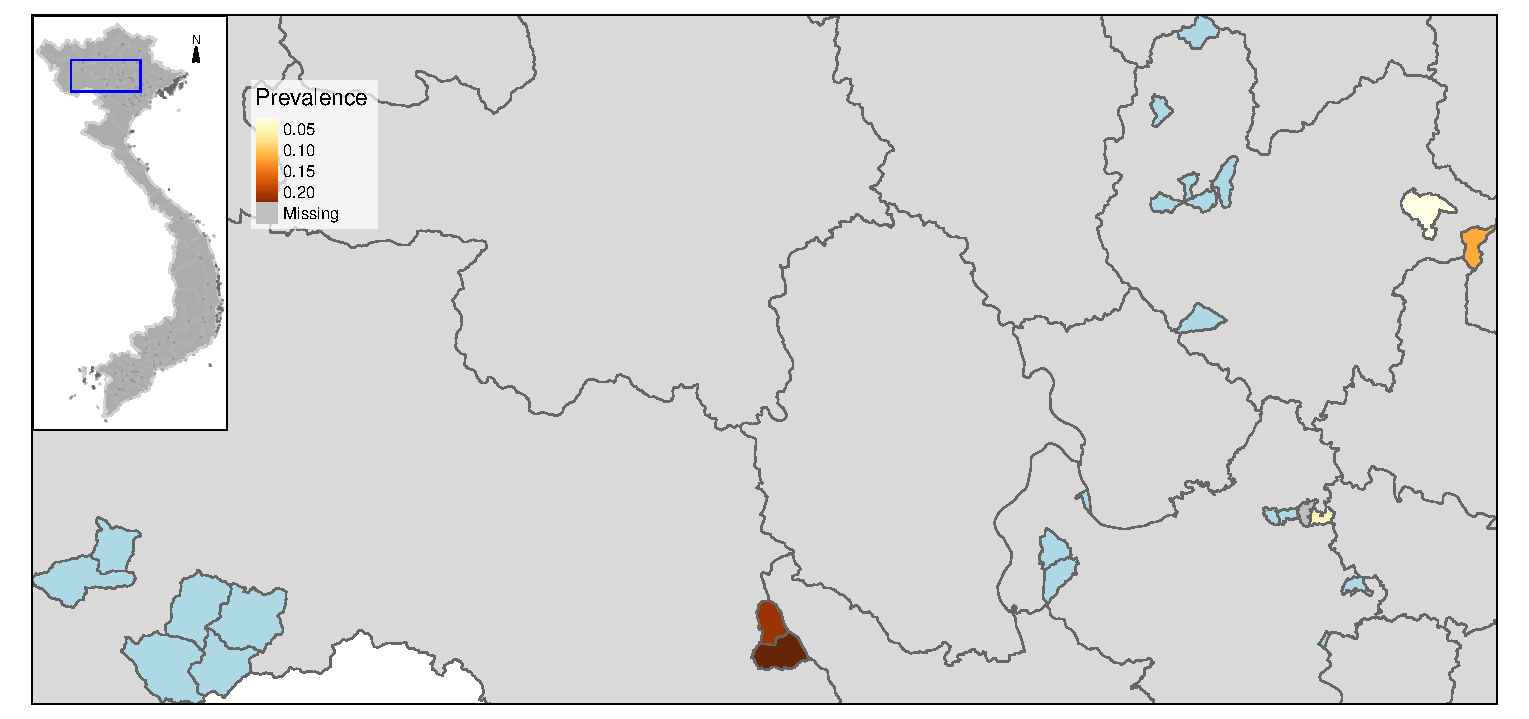
\includegraphics[width=1\textwidth]{map06_winter.pdf}
\end{center}
\end{frame}


\begin{frame}
spring\\
\begin{center}
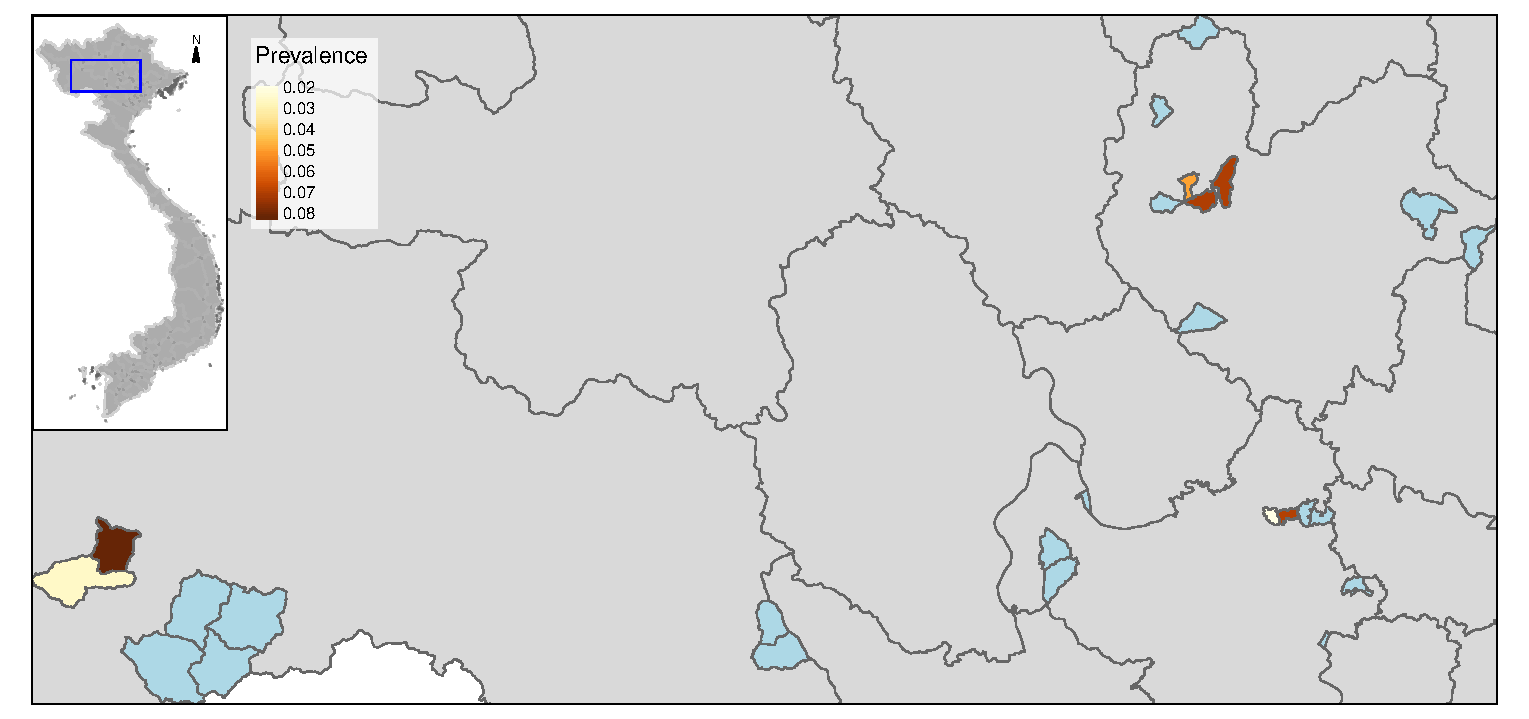
\includegraphics[width=1\textwidth]{map06_spring.pdf}
\end{center}
\end{frame}

% \begin{frame}
% \vspace{-0.6cm}
% \begin{columns}[t]
% \begin{column}{7cm}
% \begin{center}
% \includegraphics[width=1\textwidth]{figs/SI.png}\\
% Ignaz Philipp Semmelweis (1818--1865)\\
% \url{https://semmelweismuseum.hu/}\\
% {\small\url{https://www.facebook.com/SOMuseum}}
% \end{center}
% \end{column}
% \begin{column}{5cm}
% \begin{itemize}
%  \item 1847: chlorinated lime for hand washing
%  \item 1879: Pasteur presented \textit{streptococcus} from childbed fever
%  \item causality? association? efficiency
% \end{itemize}
% \vspace{1cm}
% \textit{Leviticus 13,4}:\\
% {\scriptsize%
% \textit{''If the shiny spot on the skin is white but does not appear to be more than skin deep and the hair in it has
% not turned white, the priest is to isolate the affected person for seven days.''}}
% \end{column}
% \end{columns}
% \end{frame}

\section{Metagenome}

\subsection{\textit{Musca domestica} salivary gland hypertrophy virus}
\begin{frame}
Assembly: 124,552 bp, 100 CDS (96 identified as the reference)\\
DNA polymerase (identities: 966/979 (99\%), gaps: 3/979 (0\%))\\
% {\scriptsize
% {\ttfamily
% Query  1    MLLRPNYQYNWSDDDDDDN-SVCESEQSYRSRSPSPLPWTSSSSTVTCMISDIKTQAYAN  59
%             MLLRPNYQYNWSDDDDDD+ +  ESEQSYRSRSPSPLPWTSSSSTVTCMISDIKTQAYAN
% Sbjct  1    MLLRPNYQYNWSDDDDDDSVNDNESEQSYRSRSPSPLPWTSSSSTVTCMISDIKTQAYAN  60
% Query  60   RVVNIKLSLMNEYGEKLLKLIQGDVFFDVYIETWNRNENIARILNQLQCYNNTPQFVDTK  119
%             RVVNIKLSLMNEYGEKLLKLIQGDVFFDVYIETWNRNENIARILNQLQCYNNTPQFVDTK
% Sbjct  61   RVVNIKLSLMNEYGEKLLKLIQGDVFFDVYIETWNRNENIARILNQLQCYNNTPQFVDTK  120
% Query  120  YTAMGYSQTPLNVWRLNIRENRLDYIYEFCQSSGRRMFLNTELNDALPMVQKNLGIYCDI  179
%             YTAMGYSQTPLNVWRLNIRENRLDYIYEFCQSSGRRMFLNTELNDALPMVQKNLGIYCDI
% Sbjct  121  YTAMGYSQTPLNVWRLNIRENRLDYIYEFCQSSGRRMFLNTELNDALPMVQKNLGIYCDI  180
% Query  180  PNVGDTAQIPYSSLTKPDMSTPKSFICRKLSIDIEVITPPEWTLFPDATELGCEIIIIAC  239
%             PNVGDTAQIPYSSLTKPDMSTPKSFICRKLSIDIEVITPPEWTLFPDATELGCEIIIIAC
% Sbjct  181  PNVGDTAQIPYSSLTKPDMSTPKSFICRKLSIDIEVITPPEWTLFPDATELGCEIIIIAC  240
% Query  240  TRQQDDTTTYQTDILYTDSQHREIRIENADNRNFIRFDTEYQMLEYFITSIDPHNTDLLT  299
%             TRQQDDTTTYQTDILYTDSQHREI IENADNRNFIRFDTEYQMLEYFITSIDPHNTDLLT
% Sbjct  241  TRQQDDTTTYQTDILYTDSQHREIHIENADNRNFIRFDTEYQMLEYFITSIDPHNTDLLT  300
% Query  300  GWNVRNFDLKYIYDRCCKFFPDLVAKFRQWTLDGSDISFRNVTRKGQNVTLVESFGIMIL  359
%             GWNVRNFDLKYIYDRCCKFFPDLVAKFRQWTLDGSDISFRNVTRKGQNVTLVESFGIMIL
% Sbjct  301  GWNVRNFDLKYIYDRCCKFFPDLVAKFRQWTLDGSDISFRNVTRKGQNVTLVESFGIMIL  360
% Query  360  DMYDYNKSNVKAKSYKLKDIARKYLREDKQKLDIDYKDISRFYRSGNTKEFSHLLEYCSV  419
%             DMYDYNKSNVKAKSYKLKDIARKYLREDKQKLDIDYKDISRFYRSGNTKEFSHLLEYCSV
% Sbjct  361  DMYDYNKSNVKAKSYKLKDIARKYLREDKQKLDIDYKDISRFYRSGNTKEFSHLLEYCSV  420
% Query  420  DAEIVLDLMAVQKVWNNTVSMADICHVPMNYVVNSGVMLRNTCMISQFVNEHTDYLLPYK  479
%             DAEIVLDLMAVQKVWNNTVSMADICHVPMNYVVNSGVMLRNTCMISQFVNEHTDYLLPYK
% Sbjct  421  DAEIVLDLMAVQKVWNNTVSMADICHVPMNYVVNSGVMLRNTCMISQFVNEHTDYLLPYK  480
% Query  480  HEMPFTSYEGGYVNEPIVGFHTDPIFVLDFNSLYPTTMLAFNICTTTIVDMREYSDTGYP  539
%             HEMPFTSYEGGYVNEPIVGFHTDPIFVLDFNSLYPTTMLAFNICTTTIVDMREYSDTGYP
% Sbjct  481  HEMPFTSYEGGYVNEPIVGFHTDPIFVLDFNSLYPTTMLAFNICTTTIVDMREYSDTGYP  540
% Query  540  IDAIPSTSSSSDTTPYQPTELDQVVFTTSNELKISATPYMHNVGFVAANHRRGVMPQILH  599
%             IDA+PST  SSDTTPYQPTELDQV+FTTSNELKISATPYMHNVGFVAANHRRGVMPQILH
% Sbjct  541  IDAMPST--SSDTTPYQPTELDQVIFTTSNELKISATPYMHNVGFVAANHRRGVMPQILH  598
% Query  600  NLLTTRKRLQNELKKTTDDQKRKQLDAQQLSYKLCANAIYGLLGCSFSPLYNPMVAASVT  659
%             NLLTTRKRLQNELKKTTDDQKRKQLDAQQLSYKLCANAIYGLLGCSFSPLYNPMVAASVT
% Sbjct  599  NLLTTRKRLQNELKKTTDDQKRKQLDAQQLSYKLCANAIYGLLGCSFSPLYNPMVAASVT  658
% Query  660  SFGRFLSYIKRKRITEYMAAENIEGSIVYGDTDSVMVQIRNHTIAETKAIAERYAEQVTR  719
%             SFGRFLSYIKRKRITEYMAAENIEGSIVYGDTDSVMVQIRNHTIAETKAIAERYAEQVTR
% Sbjct  659  SFGRFLSYIKRKRITEYMAAENIEGSIVYGDTDSVMVQIRNHTIAETKAIAERYAEQVTR  718
% Query  720  DIGIPPIRTEYEKIFCPFLIHKKKHYIGVMYTDNCDRHLRVEYKGNEMVRSDNCTLTTDV  779
%             DIGIPPIRTEYEKIFCPFLIHKKKHYIGVMYTDNCDRHLRVEYKGNEMVRSDNCTLTTDV
% Sbjct  719  DIGIPPIRTEYEKIFCPFLIHKKKHYIGVMYTDNCDRHLRVEYKGNEMVRSDNCTLTTDV  778
% Query  780  MRDVIDLLFFGDGDLTQKNAAITRRLEELLAEWSQLYGMYREGTPVDRELRTRVVQQAIY  839
%             MRDVIDLLFFGDGDLTQKNAAITRRLEELLAEWSQLY MYREGTPVDRELR RVVQQAIY
% Sbjct  779  MRDVIDLLFFGDGDLTQKNAAITRRLEELLAEWSQLYNMYREGTPVDRELRARVVQQAIY  838
% Query  840  SKKLAKEVYTNRLPHVAVYERMKNRKQYHIGDRIVYCIANTELSDRVKPKNIIDMAYDID  899
%             SKKLAKEVYTNRLPHVAVYERMKNRKQYHIGDRIVYCIANTELSDRVKPKNIIDMAYDID
% Sbjct  839  SKKLAKEVYTNRLPHVAVYERMKNRKQYHIGDRIVYCIANTELSDRVKPKNIIDMAYDID  898
% Query  900  EFLEDERLYLAVHYYADACVRKPLSRLFASLDSQFRTQLELTLSRLFPSLVASAQKRAHK  959
%             EFLEDE+LYLAVHYYADACVRKPLSRLFASLDSQFRTQLELTLSRLFPSLVASAQKRAHK
% Sbjct  899  EFLEDEQLYLAVHYYADACVRKPLSRLFASLDSQFRTQLELTLSRLFPSLVASAQKRAHK  958
% Query  960  DKETAVLCKQKKSCENKRQ  978
%             DKETAVLCKQKKSCENKRQ
% Sbjct  959  DKETAVLCKQKKSCENKRQ  977
% }
% }
\begin{center}
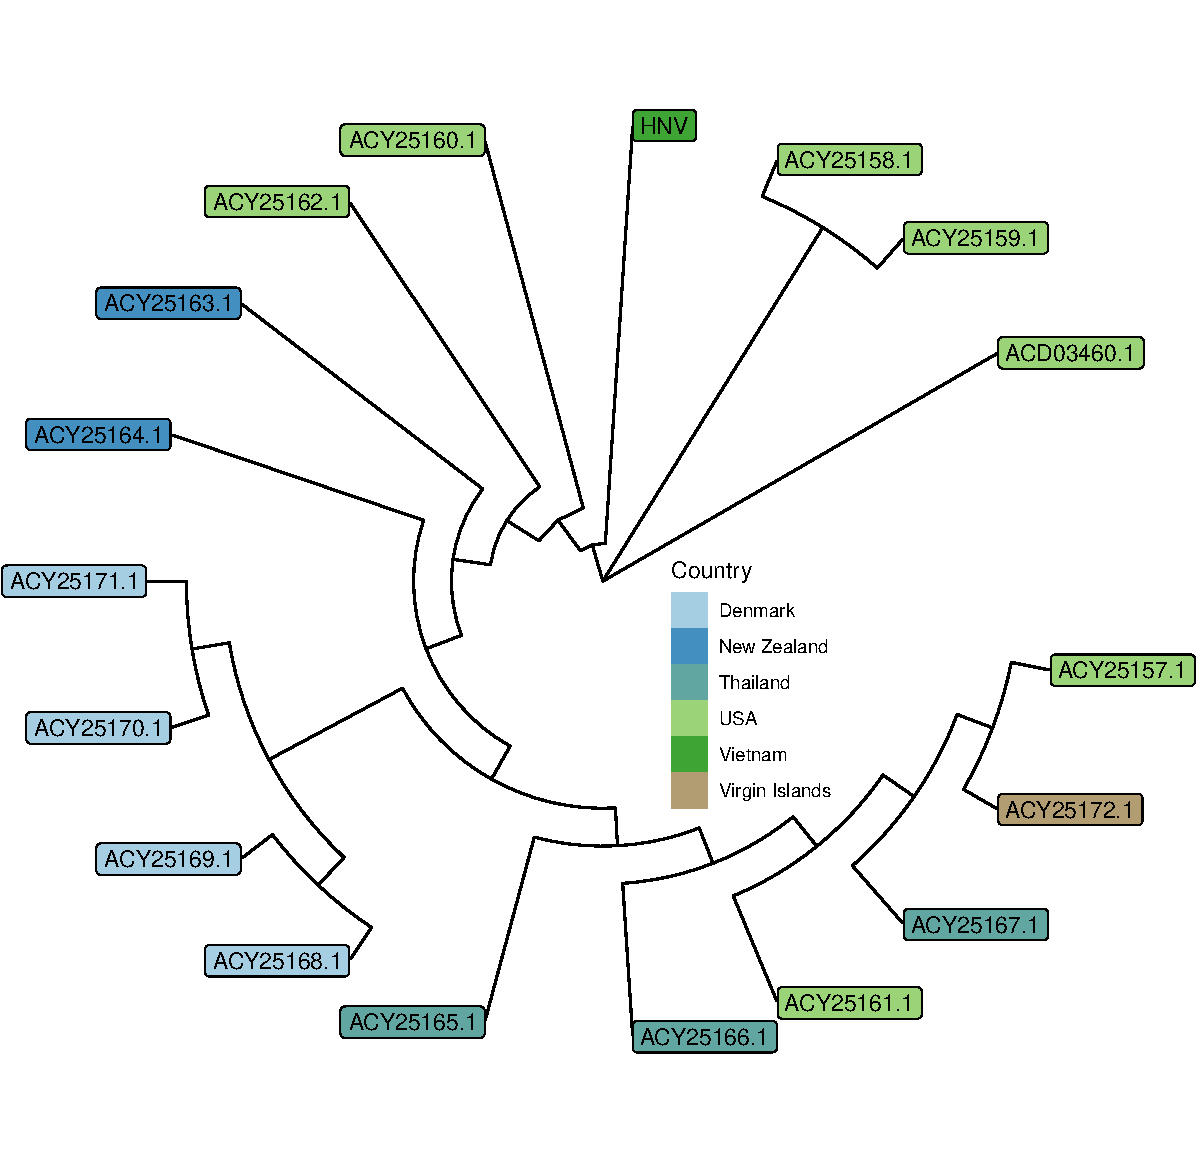
\includegraphics[trim=0cm 1.8cm 0cm 1.8cm, clip, width=0.7\textwidth]{../Viet_seq/fig_phylob.pdf}
\end{center}
\footnotetext{HNV.07, 5 NAGY secret egész}
\end{frame}

\subsection{\textit{Haematobia irritans} densovirus}
\begin{frame}
Assembly: 4,841 bp (depth 520)\\

\begin{center}
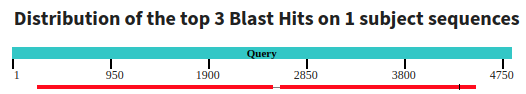
\includegraphics[width=0.8\textwidth]{../Viet_seq/HIdensovirus.png}
\end{center}

\textit{Haematobia irritans} densovirus isolate HiDV/URU, partial genome\\
4,283 bp\\
Uruguay\\
Range 1: 43 to 2329, identities: 2112/2290(92\%), gaps: 8/2290(0\%)\\
Range 2: 2326 to 4056, identities: 1517/1734(87\%), gaps: 6/1734(0\%)\\
Range 3: 4109 to 4280, identities: 156/172(91\%), gaps: 1/172(0\%)\\
\footnotetext{45-NAGY-M, 5 nagy vérszívó}
\end{frame}

\subsection{Pathogens}
\begin{frame}

\begin{center}
{\tiny%
\begin{tabular}{llrlrr}
\toprule
Sample & Contig & bp & Best match & Identities & Gaps \\
\midrule
TNV\_09 & k59\_7 & 239 & Anaplasma marginale strain Jaboticabal & 239/239 (100\%) & 0/239 (0\%)\\
 & k59\_30 & 255 & Anaplasma marginale strain Jaboticabal & 255/255 (100\%) & 0/255 (0\%)\\
HNV\_07 & k141\_5 & 307 & Trypanosoma vivax Y486 & 84/97 (87\%) & 7/97 (7\%)\\
 & k141\_10 & 349 & Leishmania amazonensis strain UA301 & 131/133 (98\%) & 0/133 (0\%)\\
 & k141\_1 & 324 & Leishmania donovani strain LdCL & 257/306 (84\%) & 2/306 (0\%)\\
 & k141\_7 & 512 & Leishmania donovani strain LdCL & 385/456 (84\%) & 0/456 (0\%)\\
 & k141\_22 & 369 &  Trypanosoma vivax Y486 & 355/369 (96\%)  & 0/369 (0\%)\\
 & k141\_4 &  397& Leishmania donovani strain Dd8 & 321/382 (84\%) & 14/382 (3\%)\\
 & k141\_14 & 742 & Trypanosomatidae sp. GMO-05 & 580/581 (99\%) & 0/581 (0\%) \\
 & k141\_18 & 1079 & Trypanosoma kuseli & 749/825 (91\%) & 19/825 (2\%)\\
 & k141\_19 & 1168 & Trypanosoma theileri YMG-11 & 1033/1141 (91\%) & 42/1141 (3\%)\\
 & k141\_20 & 1662 & Leptomonas pyrrhocoris & 1519/1666 (91\%) & 5/1666 (0\%)\\
 & k141\_21 & 3062 & Trypanosomatidae sp. GMO-05 & 1114/1120 (99\%) & 1/1120 (0\%)\\
\bottomrule
\end{tabular}
}
\end{center}
\end{frame}

% TNV_09_S2022_NAGY-M_anaplasma_final.contigs.fa
% k59_7 flag=1 multi=2.0000 len=239
% Anaplasma marginale strain Jaboticabal chromosome
% 239/239(100%)	0/239(0%)
%
% k59_30 flag=1 multi=2.0000 len=255
% Anaplasma marginale strain Jaboticabal chromosome
% 255/255(100%)	0/255(0%)
%
% HNV_07_S2022_NAGY_M_trypanosoma_final.contigs.fa
% k141_5 flag=1 multi=4.0000 len=307
% Trypanosoma vivax Y486 annotated genomic contig, chromosome 11
% 84/97(87%)	7/97(7%)
%
% k141_10 flag=1 multi=4.0000 len=349
% Leishmania amazonensis strain UA301 chromosome 27
% 131/133(98%)	0/133(0%)
%
% 141_1 flag=1 multi=4.0000 len=324
% Leishmania donovani strain LdCL chromosome LdCL_35, complete sequence
% 257/306(84%)	2/306(0%)
%
% k141_7 flag=1 multi=3.0000 len=512
% Leishmania donovani strain LdCL chromosome LdCL_15, complete sequence
% 385/456(84%)	0/456(0%)
%
% k141_22 flag=3 multi=3.0132 len=369
% Trypanosoma vivax Y486 annotated genomic contig, chromosome 11
% 355/369(96%)	0/369(0%)
%
% k141_4 flag=1 multi=3.0000 len=397
% Leishmania donovani strain Dd8 histone H3 gene, partial cds
% 321/382(84%)	14/382(3%)
%
% k141_14 flag=1 multi=6.0000 len=742
% Trypanosomatidae sp. GMO-05 small subunit ribosomal RNA gene, partial sequence
% 580/581(99%)	0/581(0%)
%
% k141_18 flag=1 multi=4.0000 len=1079
% Trypanosoma kuseli genes for IGS, 18S rRNA, 5.8S rRNA, 28S rRNA and ITS1-6
% 749/825(91%)	19/825(2%)
%
% k141_19 flag=1 multi=3.0000 len=1168
% Trypanosoma theileri YMG-11 genes for 18S rRNA, ITS1, 5.8S rRNA, ITS2, 28S rRNA, ITS3, ITS4, ITS5, partial and complete
% sequence
% 1033/1141(91%)	42/1141(3%)
%
% k141_20 flag=1 multi=6.0000 len=1662
% Leptomonas pyrrhocoris putative mitochondrial heat-shock protein hsp70 mRNA
% 1519/1666(91%)	5/1666(0%)
%
% k141_21 flag=1 multi=5.0000 len=3062
% Trypanosomatidae sp. GMO-05 small subunit ribosomal RNA gene, partial sequence
% 1114/1120(99%)	1/1120(0%)



%
% 32-NAGY-M
% 5 nagy vérszívó

% 33-NAGY-M
% 5 nagy vérszívó
%
% 34-KICSI-M
% 4 kicsi vérszívó
%
% 35-NAGY-M
% 4 nagy vérszívó
%
% 37-NAGY-M
% 1 nagy vérszívó
%
% 38-NAGY-M
% 1 nagy vérszívó
%
% 39-NAGY-M
% 1 nagy vérszívó
%
% 40-NAGY-M
% 4 nagy vérszívó
%
% 41-KICSI-M
% 4 nagy  vérszívó
%
% 41-NAGY-M
% 4 kicsi vérszívó
%
% 42-NAGY-M
% 5 nagy szekretofág
%
% 43-NAGY-M
% 5 nagy vérszívó
%
% 45-NAGY-M
% 5 nagy vérszívó
%
% 59-NAGY-M
% 5 nagy vérszívó
%
% TNV.05.S2022
% 3 NAGY secret egész
%
% körTNV.06.S2022
% 3 NAGY vérszívó egész
%
% TNV.09.S2022
% 3 NAGY vérszívó egész
%
% HNV.07.S2022
% 5 NAGY secret egész
%
% TBV.22. S 2022
% 3 KICSI egész + 1 nagy



% \input{slidesHU02}
% \input{slidesHU03}
% \input{slidesHU04}
% \input{slidesHU05}
% \input{slidesHU06}
% % % \institute[04/12/2019]{}
% \title[EBM]{Bizonyítékokra alapozott orvoslás}
% \author[QEpi]{}
% \date[]{}
% \begin{frame}[plain]
% \maketitle
% \end{frame}
% \input{slidesHU07}
% \input{slidesHU08}
% % \input{slidesHU09}
%
% \section{Ajánlott irodalom}
%
% \begin{frame}
%
% {\tiny
% \bibliography{refs}
% %
% % \nocite{Dohoo2003,Noordhuizen2001,Pfeiffer2002,Pfeiffer2010,Smith2005,
% % Thrusfield2007} %1, 2
% \nocite{Gardner2012,Stevenson2012,Noordhuizen2001,Woodworth2004,
% grimes2005refining} %3
% \nocite{messam2008frequentist,Noordhuizen2001,Gardner2012} %4
% % \nocite{Stevenson2012,Noordhuizen2001,epiR,Thrusfield2007} %5
% % \nocite{Noordhuizen2001,Stevenson2012,barratt2004tips,Dubecz2013} %6
% % \nocite{greenhalgh2010read,cockcroft2008handbook,heneghan2006evidence,
% % sanhueza2018meta,halasa2011meta,Thrusfield2007} %7
% % % \nocite{Thrusfield2007,gelman2020regression}%6-7
% % \nocite{lawson2016handbook,lawson2013statistical,lawson2013bayesian}
% }
% \end{frame}

% \input{slidesEN01}
% \input{slidesEN02}
% \input{slidesEN03}
% \input{slidesEN04}
% % \input{slidesEN05}
% % \input{slidesEN06}
% % % % % % % \institute[04/12/2019]{}
% % % % % \title[EBM]{Evidence Based Medicine}
% % % % % \author[QEpi]{}
% % % % % \date[]{}
% % % % % \begin{frame}[plain]
% % % % % \maketitle
% % % % % \end{frame}
% % \input{slidesEN07}
% \input{slidesEN08}
% % % % % % %
% %
% \section{References}
% \begin{frame}
%
% {\tiny
% %
% \bibliography{refs}
% % \nocite{Dohoo2003,Noordhuizen2001,Pfeiffer2002,Pfeiffer2010,Smith2005,Thrusfield2007} %1, 2
% \nocite{Gardner2012,Stevenson2012,Noordhuizen2001,Woodworth2004,grimes2005refining} %3
% \nocite{messam2008frequentist,Noordhuizen2001,Gardner2012} %4
% % \nocite{Stevenson2012,Noordhuizen2001,epiR,Thrusfield2007} %5
% % \nocite{Noordhuizen2001,Stevenson2012,barratt2004tips,Dubecz2013} %6
% % \nocite{greenhalgh2010read,cockcroft2008handbook,heneghan2006evidence,Patai2017,
% % sanhueza2018meta,cuzick2005forest,halasa2011meta,Thrusfield2007,
% % hothorn2014handbook} %7
% % \nocite{Thrusfield2007,gelman2020regression}%6-7
% % \nocite{lawson2016handbook,lawson2013statistical,lawson2013bayesian}
% }
% \end{frame}

\end{document}


